%%%%%%%%%%%%%%%%%%%%%%%%%%%%%%%%%%%%%%%%%%%%%%%%%%%%%%%%%%%%%%%%%%%%%%%%%%%%%%%%%%%%%%%%%%%%%%%%%%%%%%%
%%%%%%%%%%%%%% Template de Artigo Adaptado para Trabalho de Diplomação do ICEI %%%%%%%%%%%%%%%%%%%%%%%%
%% codificação UTF-8 - Abntex - Latex -  							     %%
%% Autor:    Fábio Leandro Rodrigues Cordeiro  (fabioleandro@pucminas.br)                            %% 
%% Co-autor: Prof. João Paulo Domingos Silva  e Harison da Silva                                     %%
%% Revisores normas NBR (Padrão PUC Minas): Helenice Rego Cunha e Prof. Theldo Cruz                  %%
%% Versão: 1.0     13 de março 2014                                                                  %%
%%%%%%%%%%%%%%%%%%%%%%%%%%%%%%%%%%%%%%%%%%%%%%%%%%%%%%%%%%%%%%%%%%%%%%%%%%%%%%%%%%%%%%%%%%%%%%%%%%%%%%%
\section{\esp Introdução}

As tecnologias da informação se tornaram fundamentais para o auxílio da gestão das empresas em suas atividades rotineiras e também no suporte a tomadas de decisões e possibilidade de desenvolvimento de novos modelos de negócio e a modificação dos valores estratégicos das empresas \cite{audy}.

Visando a adequação às mudanças mercadológicas, organizacionais e à manutenibilidade em relação a concorrência, o investimento em sistemas de informação tem uma grande parcela do orçamento das empresas, buscando o alinhamento da Tecnologia da informação e negócios \cite{luftman}.  
Para atender a essas necessidades, os requisitos de sistemas têm se tornado cada vez mais complexos e mutáveis diante das demandas das organizações. As denominadas metodologias ágeis permitem a entrega de software funcionais em ciclos de desenvolvimento mais curtos, considerando a velocidade demandada para a sua construção \cite{sbbrocco}. 
          
No entanto, as equipes que lidam com a infraestrutura têm a difícil tarefa de implantar um \textit{software} em produção a medida em que são criados ou modificados, pois estes sistemas requerem dependências de componentes externos, como configurações de \textit{hardware}, sistemas operacionais, banco de dados, servidores de aplicação e web e ainda configurações específicas da aplicação. Isto demanda um tempo considerável para a implantação destes sistemas\cite{sato}.

Para garantir um processo totalmente ágil e que acompanhe as exigências do negócio da organização, é necessário que haja uma integração do desenvolvimento de sistemas e as operações de infraestrutura. Portanto, essa abordagem ágil também deve ser seguida pelas equipes de infraestrutura. O movimento cultural denominado \textit{DevOps} surgido em meados de 2009 foi influenciado principalmente por metodologias ágeis e computação na nuvem. Ele teve como fundamento a automatização de processos das operações de infraestrutura e a integração entre as equipes de desenvolvimento e operações  \cite{sato}.

A automatização de processos de infraestrutura é uma das premissas do \textit{DevOps}, utilizando uma abordagem para provisionar e gerenciar recursos de computação como máquinas virtuais, discos de armazenamento, regras de segurança, instalação de \textit{software}, regras de redes e qualquer outro componente de serviço, simplificando o provisionamento e o gerenciamento de recursos. Ao tratar a infraestrutura como código, as organizações podem usar as melhores práticas de desenvolvimento de software, incluindo revisão de código e controle de versão, documentação e testes da infraestrutura. Esta abordagem reduz a complexidade do gerenciamento, pois todo o processo é dividido em tarefas  menores e  processos  mais gerenciáveis \cite{Morris:2016:ICM:3006361}.

A abordagem da infraestrutura como código, também conhecida como \textit{IaC} reduz os riscos operacionais, permitindo submeter a configuração da infraestrutura da mesma maneira que o código fonte do software é tratado, usando sistemas de gerenciamento de código-fonte, \textit{TDD} \footnote{\textit{TDD - Test Driven Development}: O teste são que são escritos antes do nosso código de produção} , integração contínua \footnote{\textit{CI - Continuous Integration}: É uma prática de desenvolvimento de software em que os desenvolvedores, juntam suas alterações de código em um repositório central e os testes são executados. Geralmente, a integração contínua se refere ao estágio de criação ou integração do processo de lançamento de software.} , refatoração de código e outras técnicas, que são úteis para garantir que as alterações na infraestrutura sejam exaustivamente testadas, repetíveis e podendo restaurar a infraestrutura em qualquer revisão anterior, quando necessário \cite{Morris:2016:ICM:3006361}.


No entanto, implantar a infraestrutura como código, pode ser uma barreira para empresas que estão migrando do modelo tradicional de infraestrutura, para uma infraestrutura baseada na nuvem, pelo fato de que os recursos (financeiro, pessoal e tempo) competem com as demandas atuais e além disso, as equipes tradicionais de infraestrutura precisam desenvolver novas habilidades, mudanças de paradigmas, como, entender os conceitos de computação na nuvem, desenvolver a habilidades de codificação em linguagens usadas pela equipe de desenvolvimento, entender de metodologias ágeis, testes, conceitos de IaC e suas ferramentas e também estabelecer um processo de gerenciamento de infraestrutura que esteja alinhado com o desenvolvimento ágil e que seja totalmente nivelado com os princípios de práticas \textit{DevOps}. 


\subsection{Problema}

O problema a ser resolvido é baseado em cenário onde uma empresa que migrou toda a arquitetura de uma aplicação comercial, baseado em \textit{Windows} para uma aplicação \textit{Web} que atualmente esta sendo desenvolvida sob a nuvem e possui uma equipe de infraestrutura que não tem conhecimento satisfatório e experiência com \textit{cloud}, não tem conhecimento em \textit{IaC} e de ferramentas de automatização de infraestrutura e um outro agravante é a competição com outras atividades, como por exemplo, gerenciamento de servidores legados o que acaba demandando muito da equipe para atender e a responder a carga de mudanças.

 A adoção de ferramentas que automatizem o provisionamento e gerenciamento de recursos, diminuíra a dependência da equipe de infraestrutura, uma vez que atualmente ela é responsável por atender demandas para a criação de atualização de recursos. Com a implantação dessas ferramentas, a equipe de desenvolvimento poderia definir os recursos durante o processo de desenvolvimento da aplicação. Neste artigo foi realizado um comparativo entre ferramentas para que auxiliem a equipe a ter um certo conhecimento e confiança para adoção de alguma ferramenta apresentada. Vale ressaltar que só adoção de uma ferramenta não resolverá o problema como um todo e essa deve ser integrada com outras ferramentas quando necessário. 

  Como motivação, tem-se os seguintes benefícios com a implantação de ferramentas:  
\begin{itemize}
 \item Eficiência no controle dos recursos, sabendo por exemplo, quais recursos uma aplicação usa;
 \item Adaptabilidade da infraestrutura aos requisitos da aplicação;
 \item Os próprios desenvolvedores podem definir , provisionar e gerenciar os recursos de que precisam, sem precisar da equipe de infraestrutura para fazer isso por eles;

\item As equipes serão capazes de se recuperar fácil e rapidamente das falhas, em vez de assumir que a falha pode ser completamente evitada;

\item Permitir a replicação parcial ou gradual da infraestrutura;

\item Permitir criar uma infraestrutura testável;
\end{itemize} 


\subsection{Objetivos}

Neste artigo serão apresentados uma abordagem geral de \textit{IaC}, um comparativo entre duas ferramentas. Os objetivos específicos serão explicar as diferenças entre softwares de gerenciamento de configuração e softwares de provisionamento, infraestrutura imutável e mutável, descrever e avaliar as características de cada ferramenta escolhida
e apresentar resultados. Este trabalho não abordará itens como: integração de ferramentas \textit{IaC}
com ferramentas de \textit{CI}, aplicações de metodologias de desenvolvimento de software.

\section{\esp Metodologia} \label{metodologia}

Para o desenvolvimento desse trabalho foram realizadas buscas sistemáticas em base  dados nacionais e internacionais pelos assuntos relacionados a estes trabalho. As bases dados utilizadas foram o \textit{IEEE}, \textit{Google Scoolar}, \textit{Carnegie Mellon University Libraries}, SciELO e portal da capes. Foram consideradas as expressões:  \textit{Infrastructure as code}, \textit{IaC}, Infraestrutura como código, \textit{Tools IaC}, \textit{Terraform}, \textit{Ansible}, Automação de infraestrutura, \textit{Infrastructure automation} , \textit{Infrastructure as code book}, \textit{Terraform book} e \textit{Ansible book}. Todos os registros de artigos publicados entre 2003 e 2019, que continham qualquer uma dessas expressões. Além disso foram pesquisadas em fontes, como livros e a documentação oficial de ferramentas estudadas neste artigo.

O motivo para estudar ferramentas de \textit{IaC} é devido a transformação causada pelo movimento Ágil, que alterou a forma como \textit{softwares} são construídos, priorizando ciclos curtos de desenvolvimento e entregas incrementais.Como resultado, a infraestrutura também passou por essa transformação, buscando a máxima disponibilidade e flexibilidade. Essa transformação veio através do movimento chamado \textit{DevOps}, que recomenda o fluxo de trabalho ágil e automatizado, e que só podem ser alcançados com a garantia de infraestrutura de TI prontamente disponível necessária para executar e testa o código desenvolvido. Isso só pode acontecer dentro de um fluxo de trabalho automatizado, o que pode ser entendido como, "Infraestrutura como código" ou IaC. As ferramentas de IaC têm um papel fundamental para criar esses fluxos de trabalhos automatizados.

Devido a isso, existe atualmente uma grande quantidade de opções de ferramentas de \textit{IaC}, que pela inexperiência da equipe no assunto, pode dificultar a escolha ferramentas que atendam o cenário ideal, que sejam fáceis de utilizar, implantar e que tenham uma integração com outras ferramentas e que garanta uma sinergia com o processo de desenvolvimento. Estabelecendo assim, um processo ágil que abrande desenvolvimento e operações de infraestrutura.  

A escolha das ferramentas obedeceram critérios da Tabela \ref{tab:tabela2} e dentre as ferramentas que atendem às características descritas nesta tabela, foram escolhidas o \textit{Ansible} e o \textit{Terraform}. Foram usados critérios extras como aceitação do mercado, suporte comercial, maturidade da ferramenta e ferramentas que trabalham no modelo de provisionamento (Abordadas na Seção \ref{tools_iac}).

Para medir a aceitação do mercado foram realizadas pesquisas em sites especializados de comparação de tipos de ferramentas e as métricas de código geradas pelo github Um outro aspecto foi certificar se é uma ferramenta \textit{open source} (um ponto importante para permitir adaptação da ferramenta), se possui um plano de suporte comercial, para critério de desempate foi considerado o preço do suporte. Para medir a maturidade foram consideradas o tempo de mercado, documentação, tempo de lançamento entre versões e a integração entre ferramentas.

Os aspectos comparativos considerados foram a linguagem de escrita, a performance (o tempo que cada ferramenta leva para criar um determinado número de recursos). O controle de estado (capacidade da ferramenta  de controlar e identificar o estado real dos recursos) e a extensibilidade da ferramenta (se possui um conjunto de \textit{SDK's} \footnote{\textit{SDK - Software Development Kit}} em que permite a programadores estender as funcionalidades da ferramenta).  Estes aspectos foram definidos de um compilado de assuntos abordados pelos autores apresentados neste artigo, como \cite{steve}, \cite{masek} e \cite{Morris:2016:ICM:3006361}.

Para a realização dos testes foram utilizados as últimas versões estáveis lançadas no momento da escrita desse artigo. A versão do \textit{Ansible} (2.4.6) e do \textit{Terraform} (0.12.13). Os testes foram realizados usando o fornecedor de computação na nuvem \textit{Digital Ocean}. \footnote{https://www.digitalocean.com/}. A escolha da \textit{Digital Ocean} é pelo fato de já ser utilizada na empresa. 

Os testes foram executados em uma máquina com um processador de 7 núcleos e 16GB de memória RAM, com o sistema operacional \textit{GNU/LINUX} com a variante \textit{UBUNTU} \footnote{https://ubuntu.com/download/desktop} na versão 18.04 no qual foi instalado as versões do \textit{Ansible} e \textit{Terraform}. Para instalar as ferramentas foi utilizado o procedimento oficial na documentação de ambas.

A execução dos foram realizadas no interpretador de linha de comandos \footnote{É uma interface baseado em texto para se interagir com o computador através de comandos} do \textit{LINUX}. Para medir o tempo de execução das ferramentas, foi utilizado o comando \textbf\textit{\textbf{time} \footnote{https://www.gnu.org/software/time/}}. Este comando mede o tempo em segundos entre início e o final de uma execução de um determinado programa. Este tempo foi convertido para minutos. Para os testes com o \textit{Ansible} foram criados 7 arquivos conforme a Tabela \ref{tab:tabela1}.

Esta tabela contém as seguintes definições:
\begin{itemize}
    \item \textbf{\textit{Nome do arquivo}}: Nome utilizado para identificar o tamanho da amostra, seguindo o padrão \textit{recurso-quantidade.yaml}
    \item \textbf{\textit{Quantidade de recursos}}: Quantidade de recursos definidos no arquivo. Para definir essa quantidade era necessário duplicar código N vezes no arquivo.
    \item \textbf{\textit{Nome do recurso}}: O nome é para garantir que seja único. Este nome foi informado no campo \textbf{\textit{name}} conforme o código da Figura \ref{fig:figura1}. 
\end{itemize}

 \begin{table}[H]
	\centering
	\caption{\hspace{0.1cm} Tabela de Recursos - Ansible}
	\vspace{-0.3cm} % espaço entre titulo e tabela
	\label{tab:tabela1}
	% Conteúdo da tabela
	\begin{tabular}{l|c|c}
  \hline
    \textbf{Nome do arquivo} & \textbf{Quantidade de recursos} & \textbf{Nome do recursos} \\
    \hline
           recurso-01.yaml   & 1  & maquina-01    \\
           recurso-02.yaml   & 2  & maquina-01, maquina-02     \\
           recurso-03.yaml   & 3  & maquina-01, maquina-nn, ..., maquina-03    \\
           recurso-05.yaml   & 5  & maquina-01, maquina-nn, ..., maquina-05       \\
           recurso-10.yaml   & 10  & maquina-01, maquina-nn, ..., maquina-10      \\
           recurso-15.yaml   & 15  & maquina-01, maquina-nn, ..., maquina-15     \\
           recurso-20.yaml   & 20  & maquina-01, maquina-nn, ..., maquina-20      \\

     \hline
 \end{tabular}
 	\vspace{.1cm}  %espaço entre tabela e fonte
	\small
	% Fonte
	{\footnotesize\\ \textbf{Fonte:  Elaborado pelo autor em 08/12/2019}}
\end{table}

\begin{figure}[H]
	\centering	
	\caption[\hspace{0.1cm} Código de definição de recurso Ansible]{Código de definição de recurso Ansible}
	\vspace{-0.4cm}
	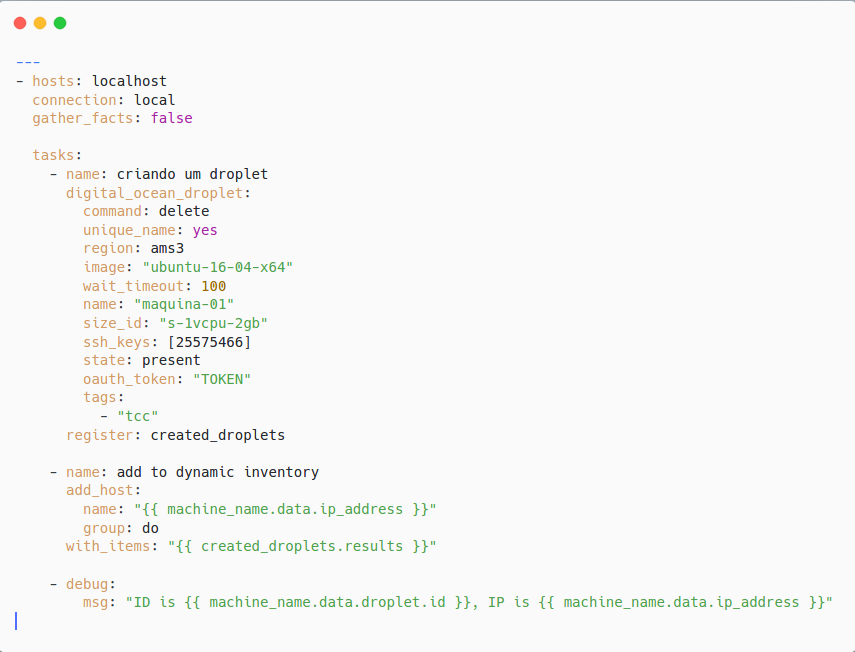
\includegraphics[width=1.0\textwidth]{artigo/figuras/codigo_ansible.png}
	 \vspace{-0.2cm}
	\\\textbf{\footnotesize Fonte: Elaborado pelo autor em 26/08/2019}
	\label{fig:figura1}
\end{figure}
\vspace{-0.5cm}

\hfill


No interpretador de comandos foi rodado o comando \textbf{\textit{time ansible-playbook -i recurso-NN.yaml}}, onde NN é o número de recursos testados. Após a execução do comando \textbf{\textit{time ansible-playbook -i recurso-NN.yaml}} era exibido o tempo total de execução pelo comando \textbf{\textit{time}}. Este tempo foi coletado e armazenado em uma planilha para compor a Tabela \ref{tab:tabela3}.

A coleta do tempo de destruição de um recurso, foi medido logo após ele ter sido criado no comando anterior. Para isso foi utilizado o comando \textbf{\textit{time ansible-playbook -i destroy.yaml}}, onde arquivo \textbf{\textit{destroy.yaml}}(veja na Figura \ref{fig:figura2}) tem os passos necessário para a destruição do recurso. Os tempo coletado foi utilizado para montar a Tabela \ref{tab:tabela4}   

\begin{figure}[H]
	\centering	
	\caption[\hspace{0.1cm} Código de destruição de recurso Ansible]{Código de destruição de recurso Ansible}
	\vspace{-0.4cm}
	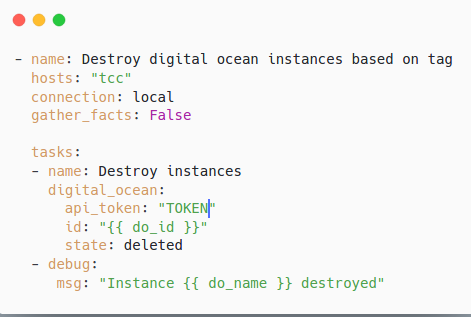
\includegraphics[width=1.0\textwidth]{artigo/figuras/destroy_codigo_ansible.png}
	 \vspace{-0.2cm}
	\\\textbf{\footnotesize Fonte: Elaborado pelo autor em 26/08/2019}
	\label{fig:figura2}
\end{figure}
\vspace{-0.5cm}

Para medir o tempo do \textit{Terraform} na criação de recursos e destruição, foram utilizados os comandos:

\begin{itemize}
    \item \textbf{\textit{time terraform init}}(Usado para download de módulos( Veja na seção \ref{terraform})).
    \item \textbf{\textit{time terraform apply droplet.tf}}, onde \textbf{\textit{droplet.tf}} é o arquivo de definição do recurso. Conforme a Figura \ref{fig:figura2}, o \textbf{\textit{count}}\footnote{count: O parâmetro count nos recursos pode simplificar as configurações permitindo dimencionar os recursos simplesmente incrementando o número. Ref: https://www.terraform.io/intro/examples/count.html }  foi incrementado com os valores 1,2,3,4,5,10,15,20. Este parâmetro define a quantidade recursos a serem criados. Após a execução do comando \textbf{\textit{time terraform apply}}, o tempo era coletado e armazenado em uma planilha para posteriormente construir a Tabela \ref{tab:tabela3}. 
    O \textbf{\textit{count}} só era incrementado após a coleta do tempo de destruição. 
    \item Para coletar o tempo de destruição o parâmetro \textbf{\textit{count}} era definido para ZERO e então o comando \textbf{\textit{time terraform destroy droplet.tf}} era rodado. Após a sua execução era exibido o tempo gasto para a execução do comando. Este tempo era armazenado em uma planilha para posteriormente construir a Tabela \ref{tab:tabela4}
\end{itemize}


\begin{figure}[H]
	\centering	
	\caption[\hspace{0.1cm} Código de Criação/destruição de recurso do Terraform]{Código de Criação/destruição de recurso do Terraform}
	\vspace{-0.4cm}
	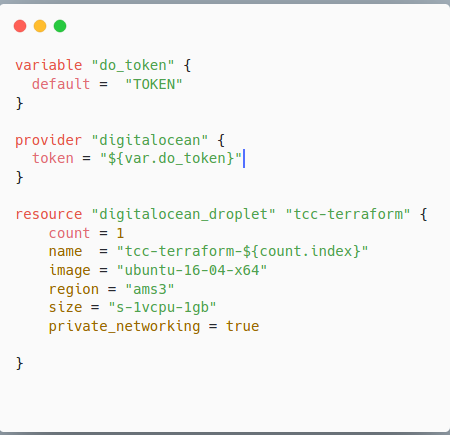
\includegraphics[width=1.0\textwidth]{artigo/figuras/terraform_resource.png}
	 \vspace{-0.2cm}
	\\\textbf{\footnotesize Fonte: Elaborado pelo autor em 30/08/2019}
	\label{fig:figura3}
\end{figure}
\vspace{-0.5cm}

 O tipo de recurso utilizado nos testes foram as máquinas virtuais. Este tipo de item é o mais utilizado na empresa.
 
 É importante destacar que para a realização dos teste é necessário ter uma na \textbf{\textit{Digital Ocean}} e um \textbf{\textit{TOKEN}} \footnote{TOKEN: É uma autorização do provedor para acessar uma API(Application Program Interface). No caso da Digital Ocean pode ser obtido por aqui: https://www.digitalocean.com/docs/api/create-personal-access-token/  }  e preencher os respectivos campos \textbf{\textit{oauth-token}} (Veja na Figura \ref{fig:figura1} e Figura \ref{fig:figura2}) e \textbf{\textit{do-token}} (Veja na Figura \ref{fig:figura3})
 
 Os testes foram realizado apenas uma vez devido ao orçamento limitado de \textbf{\$200 Dólares}.

A cotação preço do \textit{Terraform} foi obtido pelo site oficial e do \textit{Ansible} foi verificado pelo revendedor autorizado \cite{opensource.io}.

Segundo \citeonline{Guerriero} a extensibilidade de ferramenta pode ser usado fora de seu contexto original(por exemplo, fornecendo integrações com outras ferramentas e plataformas). Além disso essas ferramentas ser estendidas por meio de sistemas de \textit{plugins} e módulos. Este item foi verificado atraves da documentação oficial das ferramentas.

\section{\esp Trabalhos Relacionados} \label{relacionados}

No artigo de \cite{Guerriero} ele descreve que a metodologia \textit{DevOps} está mudando a maneira conforme \textit{Software} são desenvolvidos. O \textit{DevOps} implica em adotar um conjunto de práticas organizacionais e técnicas,por exemplo, Integração Contínua (IC), Implantação Contínua(CD), integrando as equipes de desenvolvimento e operação. Nesse contexto, a infraestrutura como código é o \textit{DevOps} na prática. A IaC é baseado em implantações na nuvem, por meio de definição de arquivos. Ele ainda cita que a computação na nuvem trouxe o provisionamento pragmático, configuração e gestão de recursos computacionais. No artigo ela faz trás dados estatísticos sobre diversas ferramentas adotadas no mercado.


\citeonline{Carnegie} explicam que o desenho da infraestrutura é a fase do ciclo de vida do produto em que se define e configura os recursos necessários para o funcionamento dele. A Infraestrutura como Código é um conjunto de práticas que usam código para configurar recursos, como máquinas e redes (virtuais), instalar programas, configurar um banco de dados e definir uma regra de segurança. As práticas IaC permitem a criação de vários recursos de maneira automatizada e padronizada, controlando o estado da infraestrutura. Além disso permitem o controle de versão, ou seja, pode-se desfazer de qualquer mudança na infraestrutura, somente alterando o código do recursos. Ele também cita que antes mesmo do surgimento da IaC os administradores de sistemas já utilizavam automação, através de \textit{script's} para realizar as tarefas de configuração de infraestrutura. E que a IaC surgiu com a popularização da computação da nuvem como serviço e que todos os recursos oferecidos são virtuais. No artigo ele ainda descreve que os provedores de serviços em nuvem fornecem um console de gerenciamento (uma interface \textit{web}) para a administração de recursos. Porém, para um sistema de larga escala, usar o console não é muito prático, devido à dificuldade de gerenciar centenas de recursos que são criados e destruídos com uma grande frequência. Deve-se usar as \textit{application program interface} \footnote{É um conjunto de rotinas e padrões de programação para acesso a um aplicativo de \textit{software} ou plataforma baseada na \textit{Web}, permitindo que dois aplicativos se comuniquem. } (API) disponibilizadas pelo provedor ou ferramentas IaC que interagem com essas API que resolvem a questão da criação e destruição de alta frequência desses recursos. Por fim, ele cita a relação entre infraestrutura como código \textit{Agile} e o DevOps. 

\hfill

Segundo \citeonline{masek}, a popularização da virtualização, o crescente poder dos servidores e a disponibilidade da computação em nuvem levaram a um aumento significativo no número de servidores e estações de trabalho que precisam ser gerenciados. Nesse ponto, as ferramentas de provisionamento e gerenciamento de configuração se aplicam nesses casos. Os administradores de sistema gerenciam grupos de servidores ou estações de trabalho idênticas (máquinas físicas ou máquinas virtuais) que executam aplicativos e serviços idênticos. Em seu artigo ele apresenta um estudo sobre o uso da ferramenta \textit{Ansible} nos laboratórios da \textit{Brno University of Technology (BUT)}. Ele descreve que o objetivo de utilizar uma ferramenta de IaC é fornecer uma plataforma para gerenciar com eficiência a infraestrutura de larga escala dos laboratórios universitários, com o mínimo de contribuição de desenvolvedores ou administradores. O autor apresenta uma Tabela \ref{tab:tabela2}, onde é mostrado dois grupos de ferramentas de infraestrutura como código mais populares: \textit{Chef, Puppet, Ansible e SaltStack, CloudWatch, Terraform, Ansible}, sendo todas “ferramentas de gerenciamento de configuração”, o que significa que elas foram projetadas para instalar e gerenciar \textit{software} em servidores e estações de trabalho já existentes. E as ferramentas  \textit{CloudFormation, Terraform} são “ferramentas de provisionamento”, o que significa que eles são projetados para provisionar os servidores.


\begin{table}[H]
	\centering
	\caption{\hspace{0.1cm} Tabela de Comparação}
	\vspace{-0.3cm} % espaço entre titulo e tabela
	\label{tab:tabela2}
	% Conteúdo da tabela
	\begin{adjustbox}{max width=\textwidth}
	\begin{tabular}{l|c|c|c|c|c|c}
  \hline
    \textbf{Itens} & \textbf{Chef} & \textbf{Puppet} & \textbf{SaltStack} & \textbf{C.Formation} & \textbf{Terraform} & \textbf{Ansible} \\
    \hline
            Open Source  & sim & sim & sim & não & sim & sim \\
            Cloud Provider & Todos & Todos & Todos & AWS & Todos & Todos  \\
            Tipo  & Config. & Config. & Config. & Provisionamento & Provisionamento & Ambas \\
            Tipo-Infra  & Mutável & Mutável & Mutável & Imutável & Imutável & Ambas  \\    
            Linguagem  & Procedural & Declarativa & Procedural & Declarativa & Declarativa & Procedural \\
            Arquitetura &  cli/server & cli/server & cliente & cliente & cliente & cliente  \\ 


     \hline
 \end{tabular}
 \end{adjustbox}
 	\vspace{.01cm}  %espaço entre tabela e fonte
	\small
	% Fonte
	{\footnotesize\\ \textbf{Adaptado de:  \cite{masek}}}
\end{table}



\hfill

 \citeonline{steve} menciona a importância de escolher ferramentas de \textit{IaC}, como por exemplo,\textit{ Chef, Ansible, Puppet, SaltStack, Terraform}. Se deve levar em consideração o conjunto de casos  que essas ferramentas se propõem a resolver. Estas são classificadas em dois domínios: gerenciamento e orquestração de configurações e quais casos elas resolvem. O autor explica os conceitos de infraestrutura mutável e imutável, escrita de código procedural e declarativa. Este conceitos serão abordados na Seção \ref{IaC}. 

\citeonline{steve} expressa que se deve escolher uma ferramenta focada na orquestração de infraestrutura e outra em gerenciamento de configuração de aplicativos reunindo os benefícios de ambas, pois os desafios do gerenciamento de provisionamento e configuração estão relacionados, porque as organizações geralmente provisionam os servidores e implantam aplicativos neles. Neste ponto os tipos de ferramentas de \textit{IaC} vão se convergir.


\section{\esp IaC ou Infraestrutura como código} \label{IaC}

Os itens apresentados neste capítulo foram levantados de acordo com assuntos abordados na Seção \ref{relacionados}. A ideia dessa seção é descrever os conceitos básicos da infraestrutura como código de forma sucinta para um entendimento geral do assunto.


\subsection{Tipos de Ferramentas IaC} \label{tools_iac}
As ferramentas de gerenciamento de configuração como \textit{Chef, Puppet, Ansible,Saltack} foram projetadas para instalar e gerenciar softwares em servidores já existentes. Por exemplo, na instalação de banco de dados, adicionar uma regra de \textit{firewall} e etc.

As ferramentas de Provisionamento como \textit{Terraform, Heat, Cloudformation} foram projetadas para criar as próprias instâncias \footnote{Uma instância é um servidor virtual na nuvem. Por exemplo: Uma instância rodando o sistema operacional LINUX} e a inicialização de seus recursos. 

Segundo \citeonline{Carnegie}, existem sobreposições e esses termos não são mutuamente exclusivos para ambas as ferramentas. As ferramentas de provisionamento podem realizar tarefas de configuração e ferramentas de configuração podem realizar tarefas de provisionamento, porém elas se concentram naquilo que são melhores. 

Ambas as categorias de ferramentas utilizam dois modelos para descrever os recursos, um tipo se concentra no resultado final, já o outro tipo descreve os passos necessários para atingir o resultado final. Este último pode ser entendido como por exemplo, comandos necessários para instalar uma versão do Java.

\subsection{Linguagem}

Segundo \citeonline{Morris:2016:ICM:3006361} as ferramentas de IaC usam arquivos de definição como \textit{DSL} \footnote{\textit{DSL - Domain-Specific Language:} Uma linguagem de domínio específico é criada especificamente para resolver problemas em um domínio particular e não se destina a ser capaz de resolver os problemas fora de seu âmbito. }, ou formatos de texto comuns conhecidos como, \textit{ YAML} \footnote{\textit{YAML - Ain't  Markup Language}: É um formato de serialização (codificação de dados) de dados legíveis por humanos -  https://yaml.org/ }, \textit{JSON} \footnote{\textit{JSON - JavaScript Object Notation:} É uma formatação leve de troca de dados. Para seres humanos, é fácil de ler e escrever. Para máquinas, é fácil de interpretar e gerar. Está baseado em um subconjunto da linguagem de programação JavaScript, https://www.json.org/json-pt.html}, \textit{XML} \footnote{\textit{XML - eXtensible Markup Language:} é uma linguagem de marcação para a criação de documentos com dados organizados hierarquicamente, tais como textos, banco de dados ou desenhos vetoriais.}
  ou linguagens de programação como, \textit{Python} \footnote{\textit{Python} é uma linguagem de programação de alto nível, interpretada, de script, imperativa, orientada a objetos, funcional, de tipagem dinâmica e forte.}  \textit{Ruby} \footnote{\textit{Ruby} é uma linguagem de programação interpretada multi-paradigma, de tipagem dinâmica e forte, com gerenciamento de memória automático.}  ou uma mesclagem de ambas.
  
  Elas se concentram em dois tipos de estilo de escrita de código: 
   \begin{itemize}
       \item Declarativo: É o modelo em que são especificados os  recursos e o estado final desejado e a própria ferramenta de Iac é responsável por descobrir como atingir este  estado estado. Veja o exemplo na Figura \ref{fig:figura4}.
   \end{itemize}

 \begin{itemize}
    \item Procedural: É o estilo na qual você escreve um código e especifica, passo a passo, como atingir o estado final desejado. O usuário deve determinar o processo de implantação ideal. Veja o exemplo na Figura \ref{fig:figura5}.
   \end{itemize}
   
 \begin{figure}[ht]
	\centering	
	\caption[\hspace{0.1cm}Exemplo declarativo]{Exemplo de escrita declarativa da ferramenta Terraform}
	\vspace{-0.4cm}
	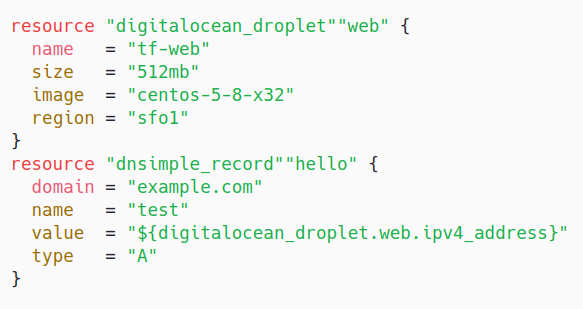
\includegraphics[width=0.98\textwidth]{artigo/figuras/terraform-declarative-exemple-01.png}
	 \vspace{-0.2cm}
	\\\textbf{\footnotesize Fonte: \cite{terraform01} }
	\label{fig:figura4}
\end{figure}
\vspace{-0.5cm}
 
\begin{figure}[h]
	\centering	
	\caption[\hspace{0.1cm}Exemplo procedural]{Exemplo de escrita procedural da ferramenta Chef}
	\vspace{-0.4cm}
	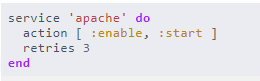
\includegraphics[width=0.5\textwidth]{figuras/chef-io-exemplo-procedural.png}
	 \vspace{-0.2cm}
	\\\textbf{\footnotesize Fonte: \cite{chef01}}
	\label{fig:figura5}
\end{figure}
\vspace{-0.5cm}

 \subsection{Tipos de Infraestrutura}
 
Nesta seção são abordadas duas características de como a infraestrutura atualmente é tratada, e apresentar uma ideia central dos conceitos. Não serão discutidos qual modelo é melhor ou quais as vantagens de se utilizar um ou outro.

Segundo \citeonline{Morris:2016:ICM:3006361}, na infraestrutura mutável, a cada mudança de algum componente, seja por uma demanda de serviço, aplicação ou segurança, as atualizações precisam ser replicadas em todos os servidores que dependem dessas mudanças. A medida que atualizações são realizadas, cada servidor tem um histórico único de alterações, possuindo sutis diferenças de configuração. As ferramentas de gerenciamento de configuração normalmente são padronizadas para este paradigma de infraestrutura mutável.

Um exemplo hipotético seria a migração do \textit{JAVA}\footnote{Java é uma linguagem de programação e plataforma computacional.} para uma versão superior. Na infraestrutura mutável cada servidor precisaria receber esta atualização do JAVA. A infraestrutura mutável é como a maioria dos ambientes computacionais funcionam hoje.
 
 Segundo \citeonline{Dadgar}, "a noção de imutabilidade é a ideia de que, uma vez criada uma coisa, não a mudamos após a criação".
 
 \hfill
 
 Na infraestrutura imutável qualquer alteração a ser realizada deve ser feita através da substituição completa dos servidores. Estas alterações são feitas criando novas configurações e novos servidores são criados a partir delas. Isso aumenta a previsibilidade porque este servidor já foi testado antes de ir para a produção. Em outras palavras, as implantações se tornam granulares. As ferramentas de provisionamento desempenham este papel \cite{Morris:2016:ICM:3006361}.
 
  Seguindo o mesmo exemplo de atualização do JAVA. Em modelo de infraestrutura imutável, um novo servidor seria criado com essa atualização e testado e então, os antigos seriam destruídos e substituídos por novos. A infraestrutura imutável só faz sentindo em um ambiente virtualizado. 
 
\subsection{Arquitetura}

Nesta seção são apresentados conceitos de como as ferramentas foram projetadas para funcionar. Não serão discutidos ou comparados qual o melhor modelo ou suas vantagens e desvantagens. 

\subsubsection{Cliente ou Masterless} \label{semagent}
Segundo \citeonline{Jan-Piet}, conforme citado por \citeonline{Morris:2016:ICM:3006361}, na arquitetura cliente não existe um servidor central e não é necessário instalar agentes nos nós gerenciados, o que torna a configuração mais simples. A configuração é feita escolhendo uma máquina e instalando o cliente e informando os IP's \footnote{\textit{Internet Protocol}} dos nós. A autenticação é feita por meio do protocolo \textit{SSH} \footnote{\textit{SSH - Sever Secure Shell:}  É um protocolo de rede criptográfico para operação de serviços de rede de forma segura sobre uma rede insegura, permitindo a execução remota de comandos.}. Ao alterar algum recurso, ele se conecta ao no \textit{IP} e executa as alterações.  Veja a Figura 6. 

\begin{figure}[H]
	\centering	
	\caption[\hspace{0.1cm}Exemplo arquitetura Cliente]{Exemplo geral de arquitetura Cliente}
	\vspace{-0.4cm}
	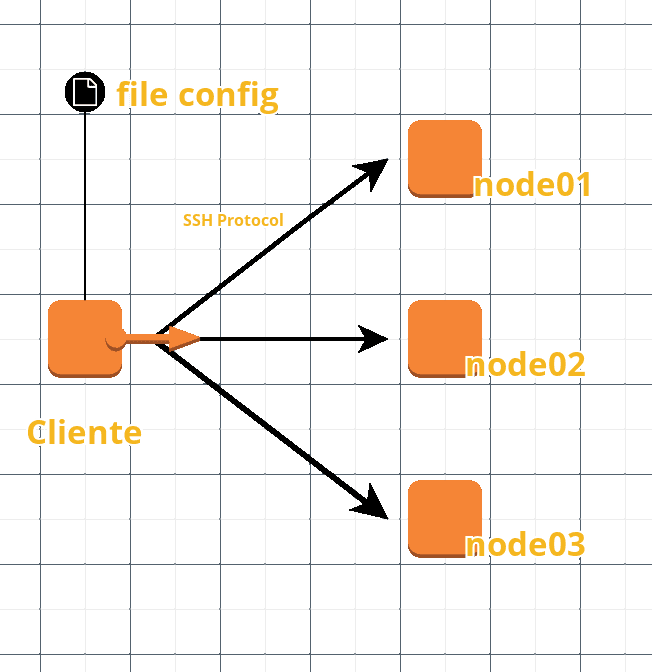
\includegraphics[width=0.5\textwidth]{figuras/cliente.png}
	 \vspace{-0.2cm}
	\\\textbf{\footnotesize Fonte: Próprio Autor}
	\label{fig:figura6}
\end{figure}
\vspace{-0.5cm}


No caso de ferramentas de provisionamento, elas se comunicam diretamente com a \textit{API} do provedor de serviços de nuvem \footnote{Um provedor de serviços de nuvem é uma empresa contratada que fornece uma plataforma, infraestrutura, aplicativo ou serviços de armazenamento baseados em nuvem. Por exemplo: \textit{Amazon Web Service, Azure, Digital Ocean, Google Cloud.}. Eles também são conhecido pelo termo \textit{IaaS - Infrastructure as a service} }


\subsubsection{Mestre/Agente ou Cliente/Servidor} \label{cliente-servidor}
 
  Nessa arquitetura (Figura \ref{fig:figura7}), um servidor \footnote{Dependendo da ferramenta o \textit{master} pode ser representado por mais de um servidor} central denominado mestre que controla as informações de configuração de cada nó(cada servidor tem instalado  um agente, geralmente rodando como um processo em segundo plano \footnote{Processos em que não há interação com o usuário}). Periodicamente, cada agente solicita informações ao mestre. O mestre gera informações e retorna um conjunto alterações desse nó. Ao receber esse conjunto com as alterações a serem realizadas, o agente aplica as alterações no nó. \cite{puppetlabs}. 
 
 Em outras palavras, o fluxo básico de funcionamento é: quando se altera as definições de um recurso, por exemplo, uma nova versão do \textit{Apache} \footnote{É um servidor \textit{web}, compatível com o protocolo HTTP, mantido pela \textit{Apache Software Foundation }}, estas são submetidas para o mestre. Quando o Agente solicita informações do mestre, o mestre retorna um conjunto com alterações para o nó desse agente. O agente recebe essas alterações e as aplica no nó correspondente, alterando a versão do \textit{Apache}.   

Segundo \citeonline{Morris:2016:ICM:3006361}, essa arquitetura pode ter uma leve variação entre ferramentas, podendo ter uma máquina exclusiva de onde o mestre é acessado.

As ferramentas que mais se enquadram a este modelo, são as de gerenciamento de configuração, como \textit{Puppet} e \textit{Chef}. Este tipo de ferramenta não será abordada neste artigo. 
 
 \begin{figure}[ht]
	\centering	
	\caption[\hspace{0.1cm}Exemplo arquitetura Master/Agent]{Exemplo geral de arquitetura Master/Agent}
	\vspace{-0.4cm}
	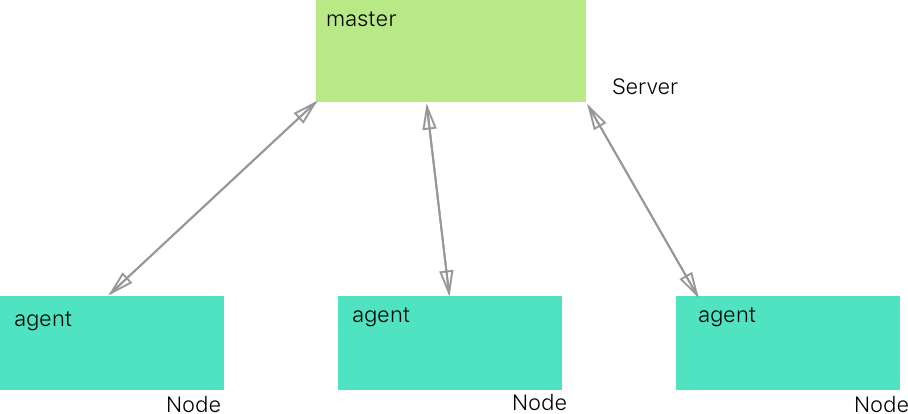
\includegraphics[width=0.5\textwidth]{figuras/master-agent.png}
	 \vspace{-0.2cm}
	\\\textbf{\footnotesize Fonte: \cite{Harit}}
	\label{fig:figura7}
\end{figure}
\vspace{-0.5cm}

\section{Ferramentas}

Esta seção aborda os principais conceitos das ferramentas utilizadas neste artigo. \textit{Ansible} e \textit{Terraform} operam usando uma arquitetura sem agente (conforme mencionado na Seção \ref{semagent}) e promovem uma interface simplificada legível para a definição de recursos, facilitando a adoção. As definições de conceitos foram retiradas diretamente da documentação oficial das ferramentas.

\subsection{Ansible} \label{Ansible}

A \citeonline{redhat} descreve o \textit{Ansible} como uma suíte completa de automação de processos de TI simples. Ele abrange desde o provisionamento e o gerenciamento de configurações e outras necessidades.

Ele não usa agentes e nenhuma infraestrutura de segurança personalizada adicional (uma característica de ferramentas, conforme mencionado na Seção \ref{cliente-servidor}), por isso é relativamente fácil de implantar. O \textit{Ansible} usa uma linguagem de marcação muito simples, o \textit{YAML}, o que é chamado como \textit{Ansible Playbooks} e o estilo de escrita de código é a procedural. E é através dos \textit{Playbooks} que se definem os recursos, sendo que estas definições se aproximam de uma escrita em inglês. \cite{redhat}.

Segundo o \citeonline{mckendrick2018learn}, o \textit{Ansible} é descentralizado e depende das credenciais existentes do sistema operacional para controlar o acesso à máquinas remotas. A principal e mais usada forma dele se conectar é usando o protocolo \textit{SSH}. Se necessário, ele pode se conectar facilmente por \textit{Kerberos} \footnote{É um protocolo desenvolvido para fornecer poderosa autenticação em aplicações usuário/servidor, onde ele funciona como a terceira parte neste processo, oferendo autenticação ao usuário.}, \textit{LDAP} \footnote{\textit{LDAP - Lightweight Directory Access:} É um protocolo de aplicação aberto para acessar e manter serviços de informação de diretório distribuído sobre uma rede de IP, permitindo o compartilhamento de informações sobre usuários, sistemas, redes, serviços e aplicações através da rede.} e outros sistemas de gerenciamento de autenticação centralizados.


\textit{Ansible} nasceu como uma ferramenta de gerenciamento de configurações e a partir da versão 2.0 passou a ser uma suíte completa, também podendo provisionar infraestrutura. Neste caso utiliza-se chamadas de \textit{API} diretamente do provedor de núvem. O \textit{Ansible} apresenta os seguintes itens em sua arquitetura: \cite{redhat}

\hfill
 \begin{itemize}
\item \textbf{\textit{Controller Machine}}: É a máquina de onde o \textit{Ansible} está sendo executado. 

\item \textbf{\textit{Modules}}: Um módulo normalmente abstrai uma tarefa do sistema, por exemplo, instalar um determinado aplicativo e o configurar. Um módulo pode ser escrito em qualquer linguagem de programação. Para usar um módulo, basta referenciar este módulo em alguma tarefa. Os módulos são executados diretamente em um nó.   

\item \textbf{\textit{Plugins}}: Os \textit{plugins} permitem estender as funcionalidades e recursos do \textit{Ansible}, por exemplo, um \textit{plugin} para o envio de \textit{e-mail}. Os \textit{plugins} devem ser escritos em \textit{Python}. Diferente dos módulos, os \textit{plugins} são executados na máquina de controle.

\item \textbf{\textit{Inventory}}: É um arquivo de configuração que contém informações sobre os nós (servidores) que o \textit{Ansible} está gerenciando. Todos os servidores gerenciados devem ser informados nesse arquivo.

\item \textbf{\textit{Playbooks}}: É o principal ponto de entrada para definir os recursos, escritos por meio do formato \textit{YAML}.

\item \textbf{\textit{Role}}: Uma maneira predefinida de organizar \textit{playbooks} e outros arquivos para facilitar o compartilhamento e a reutilização.

\item \textbf{\textit{Play}}: Uma execução de um \textit{playbook} do início ao fim.

\item \textbf{\textit{Facts}}: Variáveis globais que contêm informações sobre o sistema, como interfaces de rede ou sistema operacional.

\item \textbf{\textit{Task}}: Um bloco de código que define um único procedimento a ser executado, por exemplo, instalar o \textit{Apache}.
 \end{itemize}
 
 \begin{figure}[ht]
	\centering	
	\caption[\hspace{0.1cm}Exemplo de funcionameno do Ansible]{Exemplo de funcionameno do Ansible}
	\vspace{-0.4cm}
	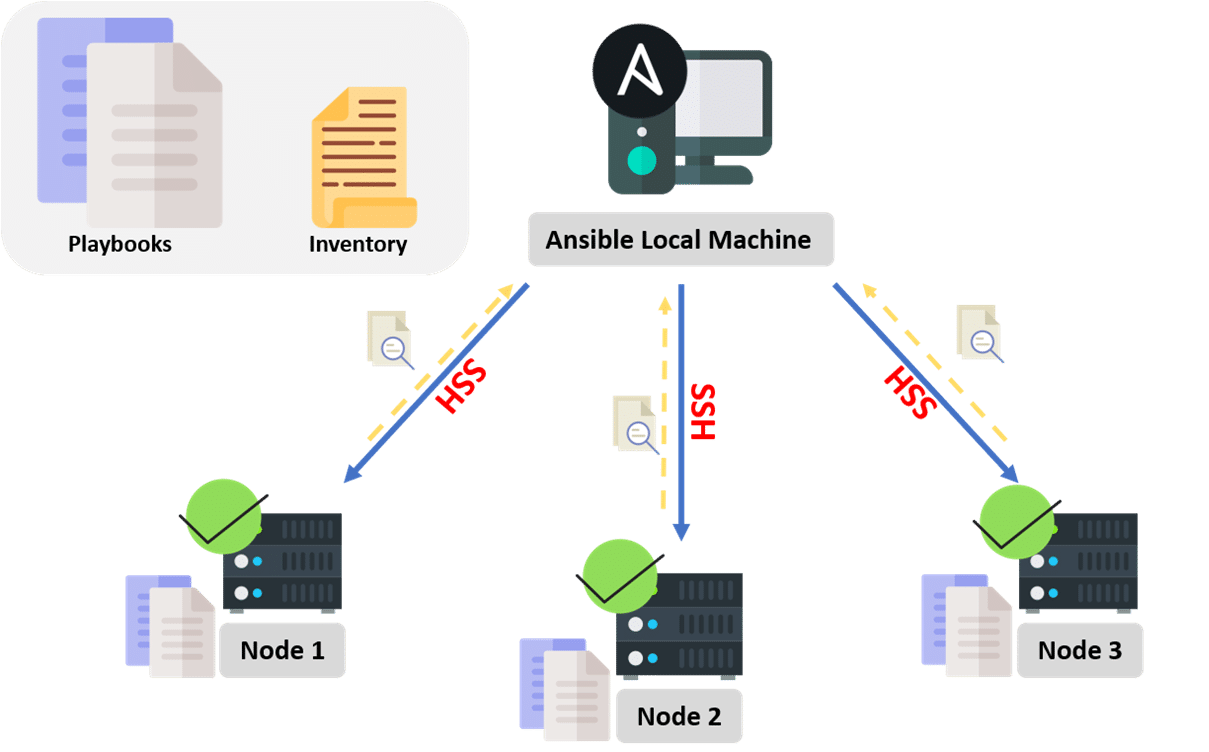
\includegraphics[width=0.5\textwidth]{figuras/ansible-working.png}
	 \vspace{-0.2cm}
	\\\textbf{\footnotesize Fonte: \cite{intellipaat}}
	\label{fig:figura6}
\end{figure}
\vspace{-0.5cm}

\subsection{Terraform} \label{terraform} 

 Segundo a \citeonline{hashcorp2}, o \textit{Terraform} é uma ferramenta para provisionamento de infraestrutura, que permite criar, alterar e criar versões de infraestrutura com segurança e eficiência. Ele pode gerenciar os mais populares provedores de nuvem e também trabalhar com soluções internas personalizadas.

O \textit{Terraform} usa uma linguagem \textit{DSL} muito simples, a \textit{HCL} \footnote{\textit{HCL - Hashicorp Configuration Language.} Veja mais em: \href{https://www.terraform.io/docs/configuration/syntax.html}{https://www.terraform.io/docs/configuration/syntax.html} } (veja na Figura \ref{fig:figura4}) com a extensão de arquivo \textit{"*.tf"} para a definição de recursos de infraestrutura. Os arquivos de configuração descrevem para o \textit{Terraform} os componentes necessários para criar um único aplicativo ou toda a configuração da infraestrutura. Ao executar, ele gera um plano de execução descrevendo o que fará para atingir o estado desejado e, em seguida, executa-o para construir a infraestrutura descrita. 
À medida que a configuração muda, ele determina o que mudou e cria planos de execução incrementais para serem aplicados.

Uma característica do \textit{Terraform} é garantir que ao executar um arquivo de definição de recursos várias vezes, o resultado será o mesmo, ou seja, é \textbf{idenpotente} \footnote{É a propriedade que algumas operações têm de poderem ser aplicadas várias vezes sem que o valor do resultado se altere após a aplicação inicial.} de uma operação. O \textit{Terraform} pode criar e gerenciar componentes de baixo nível, como instâncias de servidores, armazenamento e componentes de alto nível (aqui o \textit{Terraform} se sobrepõe com ferramentas de gerenciamento de configuração), como configurar um \textit{DNS} \footnote{\textit{DNS -Domain Name System}: É responsável por localizar e traduzir para números IP os endereços dos sites que digitamos nos navegadores.} de uma máquina \cite{brikman2017terraform}.

Além disso, conforme o \citeonline{brikman2017terraform}, o \textit{Terraform} pode ser integrado com as ferramentas de gerenciamento de configuração, como \textit{Ansible, Chef ou Puppet}.

O \textit{Terraform} apresenta os seguintes itens em sua arquitetura:
 \begin{itemize}

\item \textbf{Planos de Execução}: É uma etapa de "planejamento"  onde é gerado um plano de execução. Este  plano mostra quais os recursos que o \textit{Terraform} criará. Isso permite verificar os itens que serão criados antes de efetivamente serem criados na infraestrutura real.

\item \textbf{Grafo de Recursos}: Ele constrói um grafo de todos os recursos para paralelizar a criação e modificação de quaisquer recursos não dependentes. Por esse motivo, o \textit{Terraform} constrói a infraestrutura da maneira mais eficiente possível.

\item \textbf{Automação de Mudanças}: Conjuntos de alterações gerados automaticamente para serem aplicados à infraestrutura . Com o plano de execução e o gráfico de recursos, permmite-se saber exatamente o que o \textit{Terraform} mudará e em que ordem, evitando muitos possíveis erros humanos.

\item \textbf{Controle de Estado}: É um registro dos recursos provisionados no momento e que guardam o estado da infraestrutura e ativam o histórico das alterações incrementais. O estado pode ser armazenado remoto e localmente. O armazenamento de estado remoto permite que as equipes compartilhem o estado, evitem mais de uma alteração por vez e visualizem um histórico de todas as alterações na infraestrutura por equipe.

\item \textbf{\textit{Providers}}: Um provedor é responsável por entender as interações da \textit{API} e expor os recursos. Os provedores geralmente são serviços de \textit{IaaS},  por exemplo: \textit{Amazon
Web Service, Azure, Digital Ocean, Google Cloud, DNSimple, CloudFlare, Digital Ocean}.

\item \textbf{\textit{Resource}}: Um recurso fornecido por um provedor, por exemplo: uma instância, um disco.   

\item \textbf{\textit{Provisioners}}: Os provisionadores podem ser usados para executar ações específicas na máquina local ou remota, por exemplo copiar um arquivo da máquina local para a máquina remota.

\item \textbf{\textit{Modules}}: Um módulo é um agrupamento para vários recursos que são usados juntos. Os módulos podem ser usados para criar abstrações leves, para que você possa descrever sua infraestrutura em termos de arquitetura, em vez de diretamente em termos de objetos físicos.

\item \textbf{\textit{Variables}}: Usando um espaço reservado especial para inserir um valor calculado em uma sequência de caracteres. 

 \item \textbf{\textit{Variables output}}: Dados exportados por um módulo, que podem ser exibidos para um usuário  ou usados de forma programática por outro código \textit{Terraform}.
 
 \item \textbf{\textit{Plugins}}: O \textit{Terraform} é construído em uma arquitetura baseada em \textit{plugins}. Todos os provedores e provisionadores usados nas configurações do \textit{Terraform} são \textit{plugins}. Os usuários do \textit{Terraform} podem escrever novos \textit{plugins} para oferecer suporte às novas funcionalidades no \textit{Terraform}.
 \end{itemize}
  \cite{hashcorp2}
  \begin{figure}[H]
	\centering	
	\caption[\hspace{0.1cm}Exemplo de funcionamento do Terraform]{Exemplo de funcionamento do Terraform}
	\vspace{-0.4cm}
	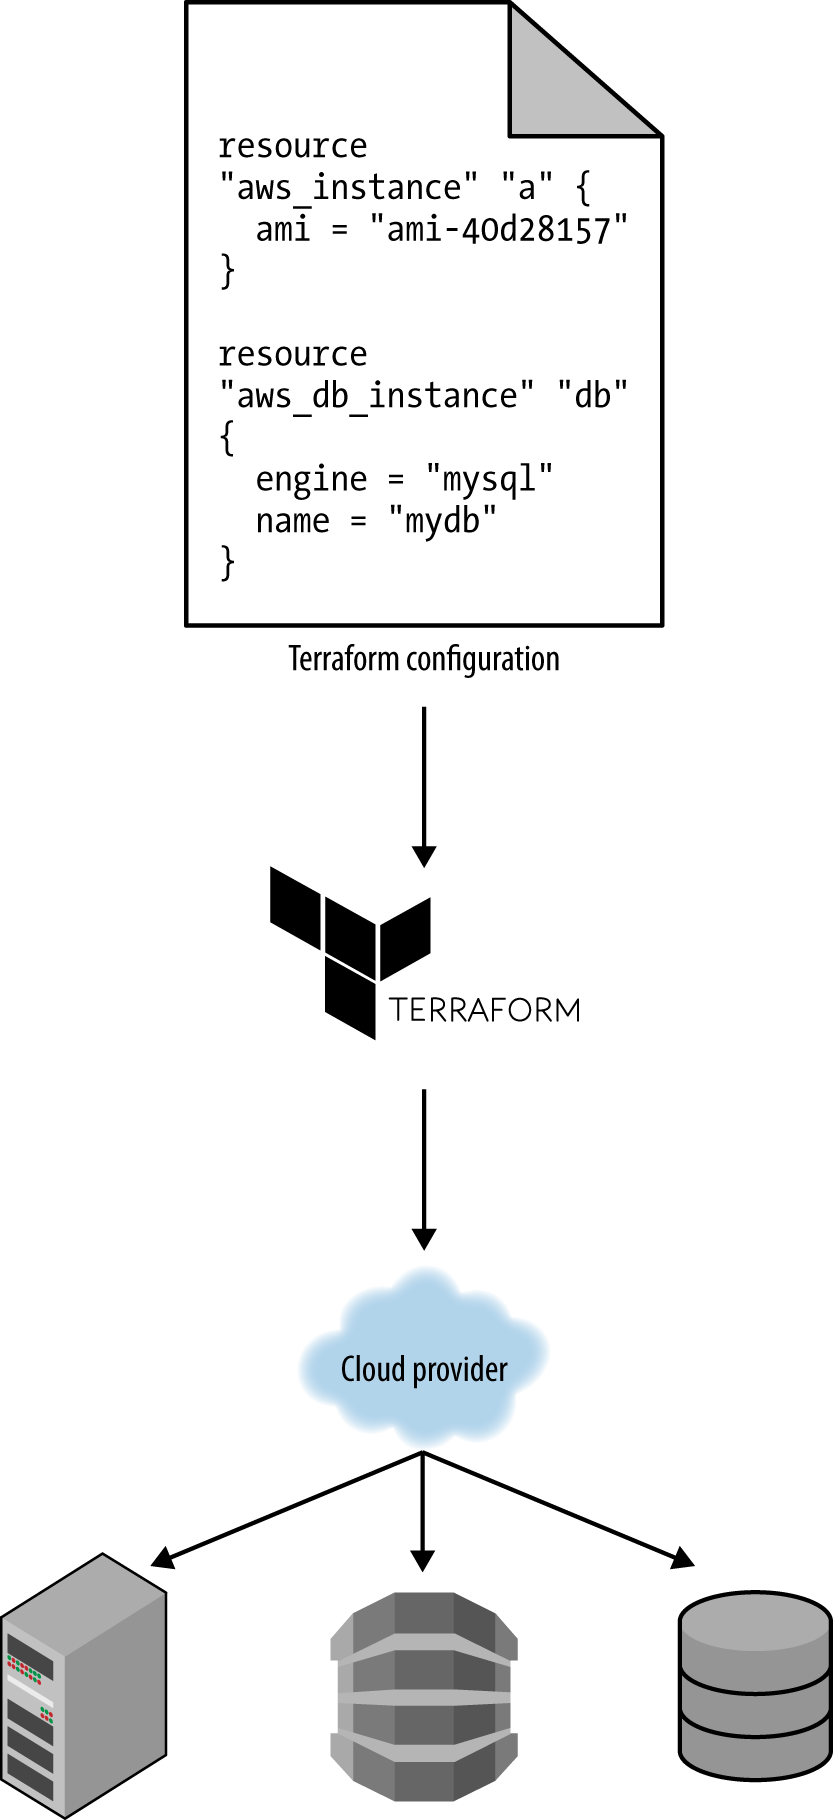
\includegraphics[width=1.1\textwidth]{figuras/terraform-working.png}
	 \vspace{-0.2cm}
	\\\textbf{\footnotesize Adaptado de: \cite{oreilly}}
	\label{fig:figura8}
\end{figure}
\vspace{-0.5cm}


\subsection{ Análise Comparativa }

Nesta seção são apresentadas diferenças entre as ferramentas, conforme descrito na Seção \ref{metodologia}, diferenças extraídas por experimentos realizados e pela análise da documentação de ambas. O intuito dessa análise é estabelecer qual ferramenta é mais fácil de implantação de utilizar.  


\subsection{Fluxo de trabalho}
Os fluxos de trabalho  das ferramentas são bem simples e atendem a equipes de diversos tamanhos. Este item descreve o fluxo principal de cada ferramenta. No fluxo de trabalho principal do \textbf {\textit{Terraform}} (veja na Figura \ref{fig:figura9}) possui três etapas: 

\begin{itemize}
  \item Definir: A definição de recursos da infraestrutura deve ser criada em qualquer editor de texto puro com a extensão \textbf{*.tf}, respeitando a sintaxe do \textit{HCL}. É prática comum armazenar os arquivos em um repositório controlado por versão.
   \item Planejar: Visualizar as alterações antes de criar os recursos (aplicar).
   \item Aplicar/Destruir: Criar, atualizar ou deletar recursos na infraestrutura. 
\end{itemize}


Este fluxo é resumido em três comandos: 


\begin{itemize}

\item \textbf{\textit{terraform init }}: Este comando é usado somente na primeira vez quando é instalado ou quando o próprio \textit{terraform} solicita. Ele realiza \textit{download} de itens de funcionamento do \textit{terraform}, como os \textit{providers, resource e modules} (\ref{terraform}). 

\item \textbf{\textit{terraform apply ou destroy }}: O terraform  detecta automaticamente as alterações de recursos, como criação, atualização e exclusão e mostra um plano do que ele fará antes de aplicar ou destruir recursos.

O \textit{Terraform} é executado por linha de comando. O usuário deve esta dentro do diretório onde possui os arquivos de definição de recursos(Conforme mencionado na Seção \ref{terraform} )  com a extensão \textbf{*.tf}, chamando o comando \textbf{\textit{terraform init}} ou \textbf{\textit{terraform apply}} ou \textbf{\textit{terraform destroy}}.  


\end{itemize}

\begin{figure}[H]
	\centering	
	\caption[\hspace{0.1cm}Fluxo Principal Terraform]{Fluxo Principal Terraform}
	\vspace{-0.4cm}
	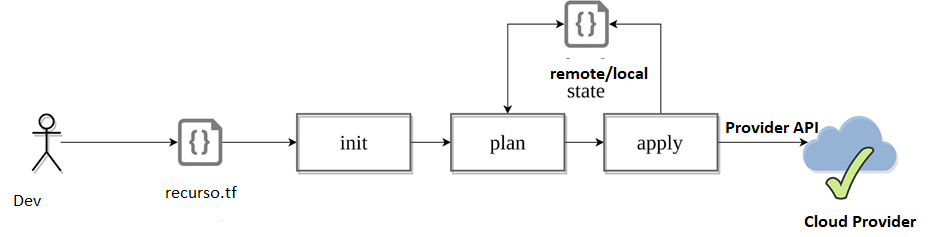
\includegraphics[width=1.0\textwidth]{artigo/figuras/terraform_single_workflow.png}
	 \vspace{-0.2cm}
	\\\textbf{\footnotesize Adaptado de: \cite{Turbinskii}}
	\label{fig:figura9}
\end{figure}
\vspace{-0.5cm}

\hfill

Considerando apenas a função de provisionamento que o \textbf{\textit{Ansible}} tem, o fluxo de trabalho também é divido em duas etapas:

\begin{itemize}
  \item Desenvolvimento: Definir os recursos da infraestrutura que devem ser criados em qualquer editor de texto puro com a extensão \textbf{*.yaml}, respeitando a sintaxe dos \textit{Playbooks}. Como no \textit{Ansible} o estado desejado deve ser descrito, deve-se definir recursos de criação, atualização e destruição.  É prática comum armazenar os arquivos em um repositório controlado por versão. 
  \item Aplicar/Destruir: Criar, atualizar ou deletar recursos na infraestrutura. 
\end{itemize}

O \textit{Ansible} é executado por linha de comando. A sintaxe para executar um \textit{playbook} é: \textbf{\textit{ansible-playbook recurso.yaml}}, onde \textit{ansible-playbook} é o nome do comando do \textit{Ansible} e \textbf{recurso.yaml} é o recurso definido pelo usuário, conforme explicado na Seção \ref{Ansible}. Veja na Figura \ref{fig:figura10} o fluxo de trabalho do \textit{Ansible}.   


\begin{figure}[H]
	\centering	
	\caption[\hspace{0.1cm}Fluxo Principal Ansible]{Fluxo Principal Ansible}
	\vspace{-0.4cm}
	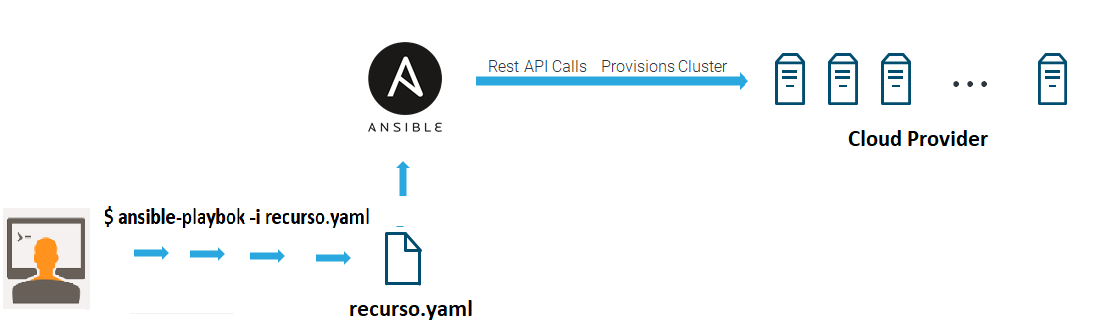
\includegraphics[width=1.1\textwidth]{artigo/figuras/Ansible_workflow2.png}
	 \vspace{-0.2cm}
	\\\textbf{\footnotesize Adaptado de: \cite{cloudera}}
	\label{fig:figura10}
\end{figure}
\vspace{-0.5cm}

\hfill

 Nesse trabalho foi usado o modo de estado local. Onde é gerado um arquivo de estado(veja na Seção \ref{terraform}) com a extensão \textbf{*.tfstate} e que deve ser armazenado no controle de versão. Outra diferença é que no \textit{Ansible} o fluxo de destruir um recursos, requer um \textit{Playbook} específico para essa finalidade. Esta última é explicada na próxima seção.  

\subsection{Controle de Estado e Idempotência} \label{idem}
Um dos grandes desafios das ferramentas de provisionamento é garantir que determinado recurso seja único e que toda operação tenha o mesmo resultado esperado, o que é chamando de idempotência tanto no \textit{Terraform} quanto \textit{Ansible}. No \textit{Terraform} isto é implícito, pois o nome associado ao recurso tem que ser único. Então, o \textit{Terraform} faz o controle automaticamente pelo nome do recurso. No \textit{Ansible} essa característica deve ser  explicitada  na definição do recurso.

Uma característica observada no \textit{Terraform} é que ele mantém o estado da infraestrutura e detecta automaticamente alterações de estado (quando um recurso foi incluído, excluído ou alterado), ele sincroniza essas diferenças entre, o estado do \textit{Terraform} e o provedor de nuvem. O \textit{Terraform} além da possibilidade do estado local, ele pode armazenar estado remoto, permitindo compartilhar o estado da infraestrutura entre equipes. Essa é uma grande vantagem em relação ao \textit{Ansible} que apresenta um modelo de recursos controlado, em que o usuário descreve o estado desejado ou seja, os passos para atingir tal estado. O que é uma grande desvantagem, pois o usuário, deve conhecer os passos necessários de como atingir o estado desejado. 

\subsection{Extensibilidade}

\textit{Ansible} e \textit{Terraform} possuem um sistema de \textit{plugins} e módulos que permite estender as suas funcionalidades. Estes módulos e \textit{plugins} são escritos em linguagens de programação e podem ser compartilhados. As duas ferramentas possuem um repositório central. No \textit{Ansible} é chamado de \textit{Galaxy}(veja na Figura \ref{fig:figura12}) e no \textit{Terraform} é chamado \textit{Registry}(veja na Figura 13). No \textit{Terraform} o usuário só pode escrever um módulo em apenas uma linguagem de programação, a \textit{Golang}  \footnote{Linguagem de programação de propósito geral desenvolvida pela Google}, e no \textit{Ansible} é permitido usar qualquer linguagem de programação.  

A vantagem de se poder usar qualquer linguagem para a extensibilidade permite-se usar uma linguagem em que uma organização já utiliza o que diminui a curva de aprendizado e evita a necessidade de aprender novas linguagens de programação.

Essa ferramentas pode ser integradas com diversos provedores de nuvem, ferramentas de controle de versão como, \textit{Github}, ferramentas de \textit{CI/CD}. 

\begin{figure}[H]
	\centering	
	\caption[\hspace{0.1cm} Interface do Ansible Galaxy]{Interface do Ansible Galaxy}
	\vspace{-0.4cm}
	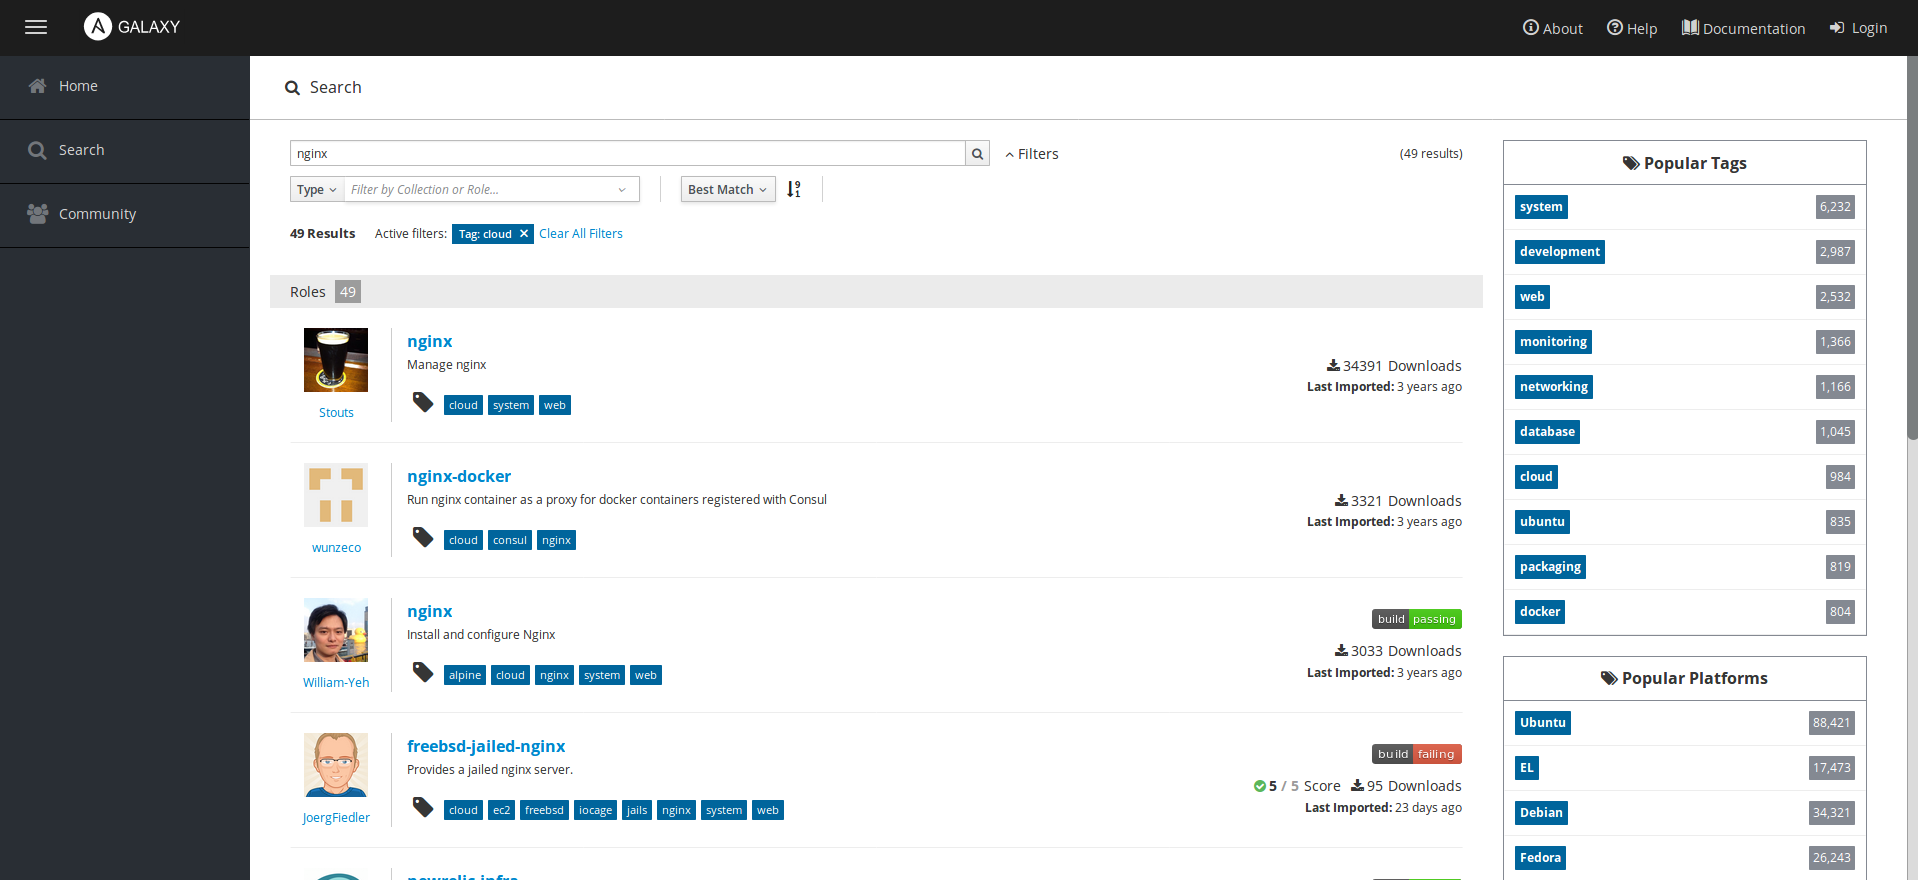
\includegraphics[width=1.0\textwidth]{artigo/figuras/galaxy_2.png}
	 \vspace{-0.2cm}
	\\\textbf{\footnotesize Fonte: \cite{ansible_galaxy}}
	\label{fig:figura12}
\end{figure}
\vspace{-0.5cm}

\begin{figure}[H]
	\centering	
	\caption[\hspace{0.1cm} Interface do Terraform Registry]{Interface do Terraform Registry}
	\vspace{-0.4cm}
	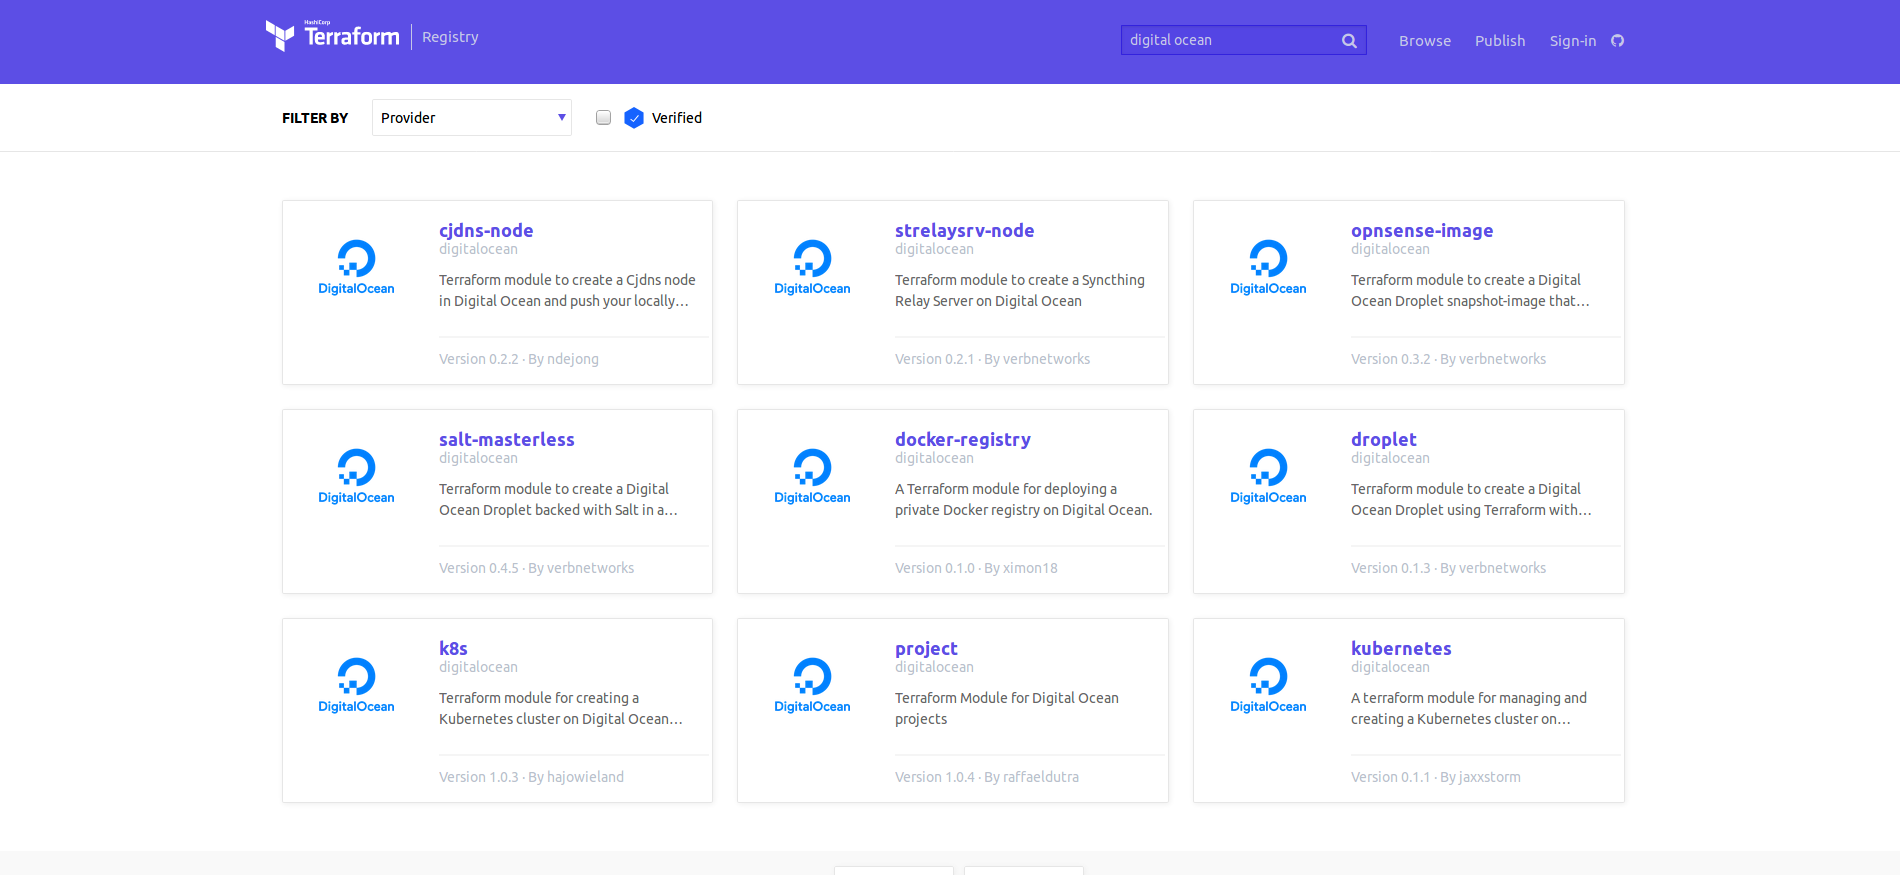
\includegraphics[width=1.0\textwidth]{artigo/figuras/terraform_registy.png}
	 \vspace{-0.2cm}
	\\\textbf{\footnotesize Fonte: \cite{terraform_registry}}
	\label{fig:figura13}
\end{figure}
\vspace{-0.5cm}

\hfill


\subsection{Performance}
Na medida em que sistemas se desenvolvem as quantidades de recursos requeridos podem aumentar ou diminuir. A velocidade em que esses recursos são criados, destruídos ou atualizados, podem por exemplo, ocasionar instabilidades, quedas de serviços, comprometendo o \textit{SLA} \footnote{ \textit{SLA}: Acordo de Nível de Serviço} de um sistema. É importante garantir que mudanças na infraestrutura sejam simples e rápidas. Um software de provisionamento deve ser eficaz a ponto de não prejudicar toda atualização de recurso \cite{sre_google}. Neste trabalho a medição da performance foi dada pelo tempo em minutos em que um recurso (utilizou-se apenas máquinas virtuais que é o recurso mais criado) foi criado no fornecedor de computação na nuvem. As Tabelas \ref{tab:tabela3} e \ref{tab:tabela4} mostram uma comparação entre \textit{Ansible} e \textit{Terraform}. 
Os dados dessas tabelas foram extraídos conforme a metologia apresentada na Seção \ref{metodologia}.

% Tabela
\begin{table}[H]
	\centering
	\caption{\hspace{0.1cm} Comparativo - Criação de MV}
	\vspace{-0.3cm} % espaço entre titulo e tabela
	\label{tab:tabela3}
	% Conteúdo da tabela
	\begin{tabular}{l|c|c}
  \hline
    \textbf{Qtde. Recursos}	& \textbf{Tempo - Ansible} & \textbf{Tempo - Terraform} \\
    \hline
  1   & 1.5 min   & 0.4  min    \\
2   & 2.10  min   & 1.5  min    \\
3   & 3.17  min   & 2.1  min    \\
5   & 5.32  min   & 4.7  min     \\
10  & 10.3  min   & 5.2  min      \\
15  & 13.8  min   & 5.7  min      \\
20  & 16.6  min   & 7.38 min      \\

     \hline
 \end{tabular}
 	\vspace{.1cm}  %espaço entre tabela e fonte
	\small
	% Fonte
	{\footnotesize\\ \textbf{Fonte:  Elaborado pelo autor em 10/11/2019}}
\end{table}


% Tabela
\begin{table}[H]
	\centering
	\caption{\hspace{0.1cm} Comparativo - Destruição de MV}
	\vspace{-0.3cm} % espaço entre titulo e tabela
	\label{tab:tabela4}
	% Conteúdo da tabela
	\begin{tabular}{l|c|c}
  \hline
    \textbf{Qtde. Recursos}	& \textbf{Tempo - Ansible} & \textbf{Tempo - Terraform} \\
    \hline
  1   & 1.2  min   & 0.4  min    \\
2   & 1.9    min   & 1.2  min    \\
3   & 2.5    min   & 1.6  min    \\
5   & 3.6    min   & 2.7  min     \\
10  & 4.20   min   & 3.2  min      \\
15  & 5.8    min   & 4.19 min      \\
20  & 7.4    min   & 5.1  min      \\

     \hline
 \end{tabular}
 	\vspace{.1cm}  %espaço entre tabela e fonte
	\small
	% Fonte
	{\footnotesize\\ \textbf{Fonte: Elaborado pelo autor em 13/11/2019}}
\end{table}


A título de comparação, para se criar uma máquina virtual no console do fornecedor, leva-se um tempo estimado de 2 min para escolher os requisitos da máquina, como sistema operacional, quantidade de memória RAM, tamanho e tipos de disco rígidos. 

Nesta comparação o \textit{Terraform} tem uma melhor performance, tanto para criação quanto para destruição de recursos. Um fato que explica essa diferença de performance é a distribuição das execuções (criação ou destruição de recursos) por núcleo. 

Segundo a \citeonline{hashcorp03}, "nossa regra prática é 10 execuções \textit{Terraform} por núcleo de CPU, com 2 núcleos de CPU alocados para os serviços básicos.  Portanto, uma máquina de 8 núcleos com 8 GB de memória pode executar confortavelmente 20 execuções \textit{Terraform}.

A comparação máxima realizada nesse trabalho ficou limitada em 20 máquinas virtuais, devido aos valores em dólares disponíveis para a realização dos testes. Entretanto, nas Tabelas 1 e 2, pode-se perceber a evolução do tempo necessário quando se aumenta a quantidade de recursos, apresentados de 1 a 20 máquinas virtuais.

\subsection{Outras Comparações}
\textit{Ansible} e \textit{Terraform} são ferramentas de código aberto e o código fonte delas está hospedado no \textit{Github}. O \textit{github} é um repositório central de código fonte, onde existem atualmente mais de 40 milhões de usuários e mais de 10 milhões de projetos e pessoas do mundo inteiro, que podem contribuir com projetos de código aberto. 

Com base nos valores indicados pelo \textit{Github}, é ainda possível extrair os seguintes aspectos comparativos: 

\begin{itemize}
    \item  Contribuidores (\textit{Contributors}): número de pessoas que contribuíram de alguma forma no projeto, corrigindo \textit{bugs}, adicionando novas funcionalidades.
     \item Frequência de atualização do código (\textit{Code Frequency}): número de linhas de código inseridas no código fonte principal anualmente. 
     \item Estrelas(stars): Quantidade de Pessoas que curtiram o projeto.
\end{itemize}

Esses aspectos são apresentados na Tabela 3.

 
   \begin{table}[H]
	\centering
	\caption{\hspace{0.1cm} Indicadores do Github}
	\vspace{-0.3cm} % espaço entre titulo e tabela
	\label{tab:tabela5}
	% Conteúdo da tabela
	\begin{tabular}{l|c|c}
  \hline
    \textbf{Métrica}	& \textbf{Ansible} & \textbf{Terraform} \\
    \hline
  Contributors & 4.752  & 1351\\
  Code Frequency(2018)  & 200MIL  &   100MIL  \\
  Stars & 40.8 MIL & 19.9MIL \\
     \hline
 \end{tabular}
 	\vspace{.1cm}  %espaço entre tabela e fonte
	\small
	% Fonte
	{\footnotesize\\ \textbf{Fonte: Elaborado pelo autor em 13/11/2019 com base nos dados do \textit{Github}}}
\end{table}

Os aspectos comparativos obtidos a partir dos dados do \textit{Github} demonstram que essas ferramentas são projetos bem consolidados e bem aceitas no mercado. O número de contribuidores e a frequência de alteração no código mostra a maturidade dos projetos e que ambos estão em evolução constante. Segundo \cite{Guerriero}, a maturidade de um projeto pode ser verficado, por exemplo, à estabilidade da ferramenta, a adoção pela comunidade(por exemplo, tendo repositórios ativos no \textit{Github} ou em um grande número de colaboradores) 

Além disso, essas ferramentas são mantidas por empresas bem avaliadas no mercado.  

Uma outra caracteristica observada são as versões das ferramentas \textit{Ansible} e \textit{Terraform} com suporte comercial. O \textit{Ansible Tower} é uma interface \textit{Web} que visa simplificar o uso do \textbf{Ansible}. Nele é possível executar \textit{playbook} e visualizar os status das tarefas concluídas. O \textit{Tower} pode ser integrado com diversas ferramentas de desenvolvimento de \textit{Software} como, controle de versões, \textit{CI/CD}. O \textit{Terraform Cloud} é uma interface \textit{web} que permite gerenciar as execuções do \textit{Terraform} em ambiente consistente e confiável com compartilhamento de estado e controles de acesso. O \textit{Terraform Cloud} pode ser integrado com diversas ferramentas.  A Tabela \ref{tab:tabela6} mostra a comparação de preços entre as ferramentas. 

   \begin{table}[H]
	\centering
	\caption{\hspace{0.1cm} Comparação de Preços}
	\vspace{-0.3cm} % espaço entre titulo e tabela
	\label{tab:tabela6}
	% Conteúdo da tabela
	\begin{tabular}{l|c|c}
  \hline
    \textbf{Produto}	& \textbf{Preço em dólar} & \textbf{Modelo de Cobrança} \\
    \hline
  Terraform Team & 20  & Usuário\\
  Terraform Team-Governace  & 70 &   Usuário  \\
  Ansible Tower  & 50-175 &   Máquina  \\
     \hline
 \end{tabular}
 	\vspace{.1cm}  %espaço entre tabela e fonte
	\small
	% Fonte
	{\footnotesize\\ \textbf{Fonte: Elaborado pelo autor em 19/11/2019 com base nos dados de \textit{\cite{opensource.io}} e  \textit{\cite{hashcorp3}}}}
\end{table}

A diferença entre os produtos é que o \textit{Ansible Tower} (Veja na Figura \ref{fig:figura13}.) deve ser instalado na infraestrutura local, já o \textit{Terraform Cloud} (Veja na Figura \ref{fig:figura14})  é uma aplicação hospedada pela \textit{Hashcorp} (empresa criadora do \textit{Terraform}). É importante salientar que o \textit{Terraform} também possui um produto com o \textit{Terraform Enterprise} que é semelhante ao \textit{Terraform cloud} e  que pode ser instalada em uma infraestrutura local, semelhante ao \textit{Ansible Tower}. No entanto, não foi possível obter valores de licenciamento desta versão.  


A Tabela \ref{tab:tabela7} mostra uma simulação  do custo de obtenção das ferramentas nas versões comerciais, considerando o menor valor de ambas. A diferença de preço entre as ferramentas chega a ser 150\% . Neste aspecto o \textit{Terraform} tem um modelo de licenciamento bem mais vantajoso que o \textit{Ansible}.  


   \begin{table}[H]
	\centering
	\caption{\hspace{0.1cm} Simulação de Preços}
	\vspace{-0.3cm} % espaço entre titulo e tabela
	\label{tab:tabela7}
	% Conteúdo da tabela
	\begin{tabular}{l|c|c|c}
  \hline
    \textbf{Produto} & \textbf{Preço em Dólar} & \textbf{Quantidade}  & \textbf{Valor total em Dólar} \\
    \hline
  Terraform Team & 20  & 10 & 200\\
  Ansible Tower  & 50 & 10 & 500\\
     \hline
 \end{tabular}
 	\vspace{.1cm}  %espaço entre tabela e fonte
	\small
	% Fonte	
	{\footnotesize\\ \textbf{Fonte: Elaborado pelo autor em 19/11/2019 com base nos dados da Tabela \ref{tab:tabela6}}}
\end{table}

\begin{figure}[H]
	\centering	
	\caption[\hspace{0.1cm} Interface do Ansible Tower]{ Interface do Ansible Tower}
	\vspace{-0.4cm}
	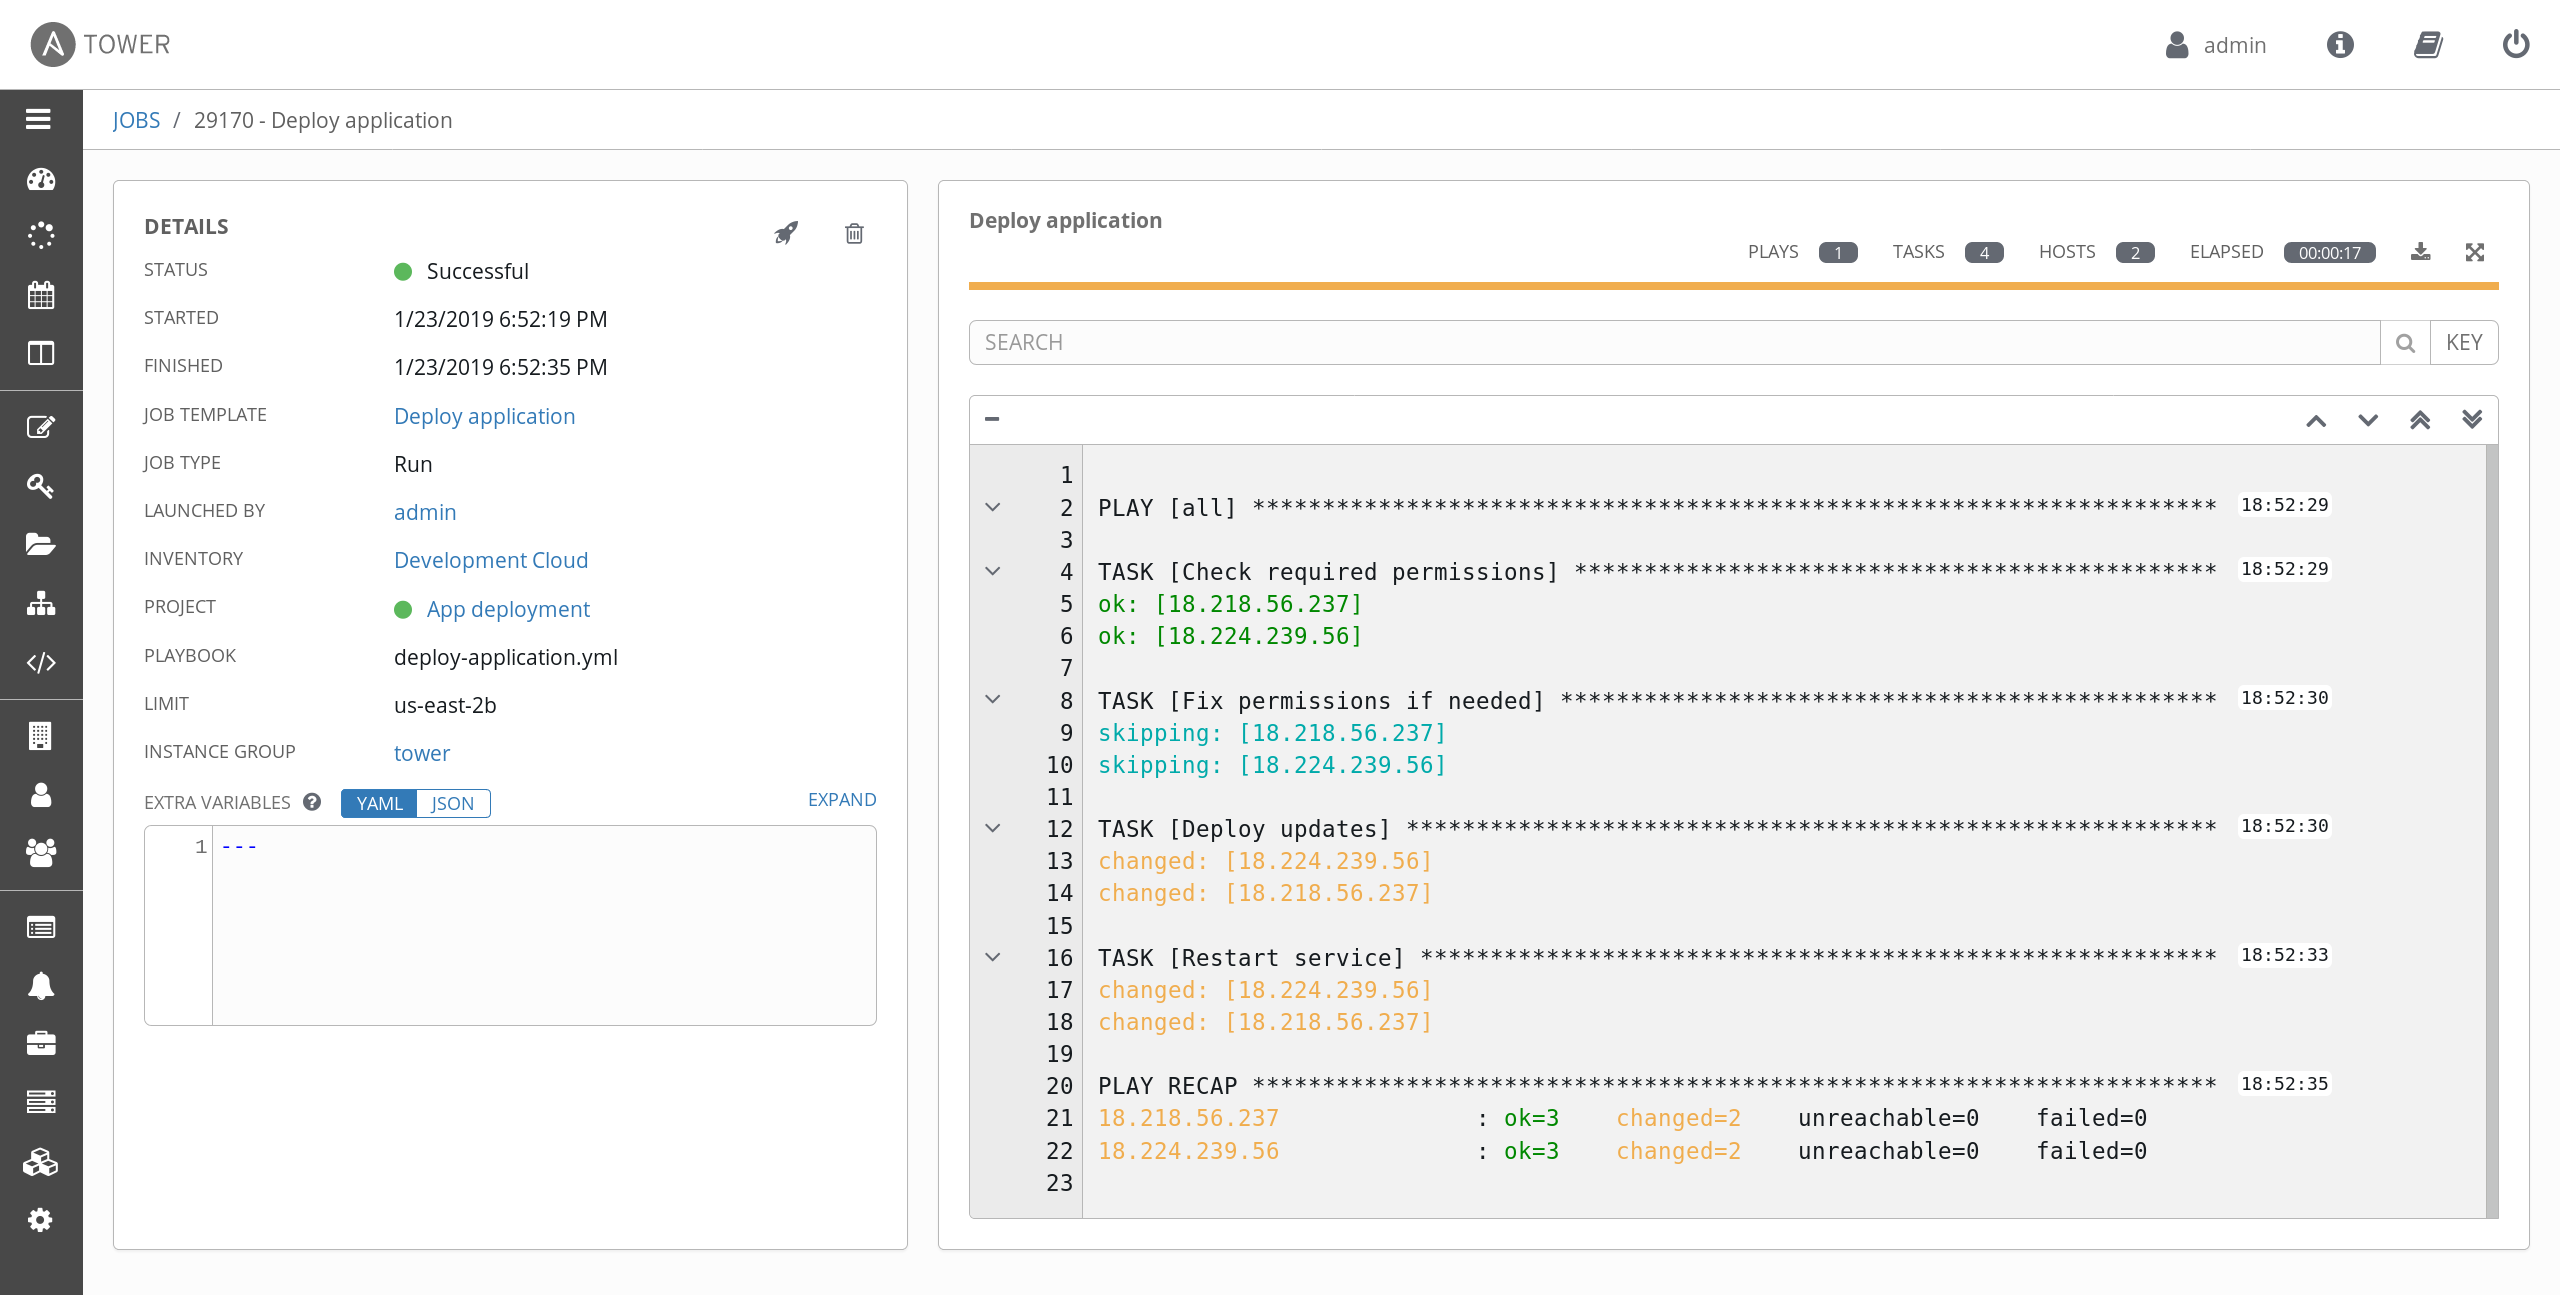
\includegraphics[width=1.0\textwidth]{artigo/figuras/RH-Ansible-Tower-job-details.png}
	 \vspace{-0.2cm}
	\\\textbf{\footnotesize Fonte: \cite{ansible_tower}}
	\label{fig:figura13}
\end{figure}
\vspace{-0.5cm}

No entanto, os modelos de licenciamento são diferentes, uma ferramenta licencia por usuário e a outra  por máquina. É importante destacar que deve-se avaliar outros aspecto,s o que significa que um modelo não é mais vantajoso que o outro. 

\begin{figure}[H]
	\centering	
	\caption[\hspace{0.1cm} Interface do Terraform Cloud]{ Interface do Terraform Cloud}
	\vspace{-0.4cm}
	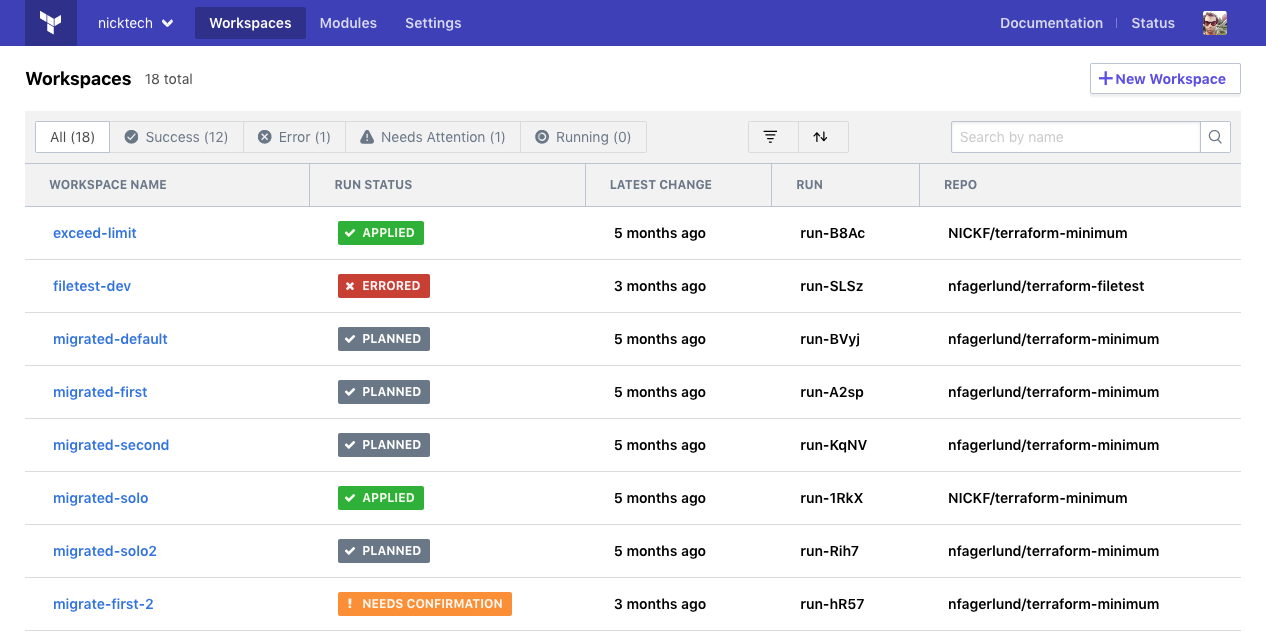
\includegraphics[width=1.0\textwidth]{artigo/figuras/terraform_cloud.png}
	 \vspace{-0.2cm}
	\\\textbf{\footnotesize Fonte: \cite{terraform_cloud}}
	\label{fig:figura14}
\end{figure}
\vspace{-0.5cm}

\hfill

\subsection{Conclusão}
Na infraestrutura como código (IaC), todos os recursos, como rede, máquinas virtuais, bancos de dados e outros, são descritos em uma linguagem de alto nível. A IaC contribui com muitos benefícios, como por exemplo: criar uma infraestrutura dinâmica, onde recursos podem ser facilmente criados, destruídos ou substituídos. Além disso, essa infraestrutura é reproduzível e testável, já que os recursos podem ser aplicados novamente em uma infraestrutura auxiliar. Ela é escalável, uma vez que os recursos podem ser redimensionados de acordo com as necessidades, alterando apenas o código do recurso. É possível realizar a rastreabilidade, uma vez que os recursos definidos podem ser versionado, seguindo o mesmo fluxo de desenvolvimento de um sistema, por exemplo.

Na análise comparativa dessas ferramentas, foi observado que o \textit{Terraform} é uma ferramenta que se destaca pelo fato de gerenciar o estado da infraestrutura automaticamente. Outro aspecto observado foi a linguagem definição de recursos ser de alto nível, sendo esse um grande diferencial da ferramenta, pois o gerenciamento de código se torna simples, uma vez que não é necessário conhecer os passos para se chegar ao estado final desejado. Por outro lado,  

Um ponto observado do \textit{Ansible} é que apesar de ser uma suíte completa para se trabalhar com infraestrutura, ele muitas vezes é indicado para se trabalhar em conjunto com ferramentas de provisionamento \textit{Terraform}.  
Outro ponto é a velocidade de manipular recursos tanto na sua criação quanto na destruição. 

 Uma outra vantagem é o \textit{Terraform Cloud} que é disponibilizado no modelo de \textit{SaaS}, o que significa software como serviço. Este modelo é vantajoso porque se permite a redução de infraestrutura e manutenção, ter uma alta disponibilidade e apenas se preocupar com a infraestrutura do negócio, visto que não será necessário gerenciar um servidor de \textit{Terraform}. Em contraponto com \textit{Ansible Tower} que deve ser instalado na infraestrutura local, o que reflete no aumento da infraestrutura para se manter o negócio, o aumento de licenças de software, além de ter mais um servidor apenas para gerenciá-la. 

O \textit{Terraform} sem dúvidas é uma ferramenta que melhor se encaixa em um cenário de infraestrutura como código, pelo fato da ferramenta já ter sido pensada para essa finalidade. Além dos benefícios da infraestrutura como código, ela traz novas abordagens, como por exemplo: a infraestrutura imutável, abordada nesse trabalho.

É importante destacar que apenas ferramentas, como \textit{Ansible} ou \textit{Terraform}, não resolvem todos os problemas, sendo necessário utilizá-las em conjunto com outras.\cite{Guerriero}. Porém, é um ponto de partida para iniciar a implantação de um modelo baseado em infraestrutura como código e obter os benefícios indicados nesses artigo.

Como trabalhos futuros, pode-se fazer uma análise criteriosa que avalie se é vantajoso ou não o uso de infraestrutura imutável. Além disso, pode-se incluir a análise de outras ferramentas de IaC, tais como a \textit{Packer} \footnote{https://www.packer.io}. 
Como as equipes de infraestrutura não possuem atualmente experiência com IaC, não existe uma análise que indique para as organizações o custo/benefício do uso de infraestrutura como código (IaC). Dessa forma, um outro trabalho seria a análise financeira da economia que poderia ser gerada com o emprego da infraestrutura como código.





